
%%%%%%%%%%%%%%%%%%%%%%%%%%%%%%%%%%%%%%%%%%%%%%%%%%%%%%%%%%%%%%%%%%
\section{Advanced control topics}
%%%%%%%%%%%%%%%%%%%%%%%%%%%%%%%%%%%%%%%%%%%%%%%%%%%%%%%%%%%%%%%%%%


%%%%%%%%%%%%%%%%%%%%%%%%%%%%%%%%%%%%%%%%%%%%%%%%%%%%%%%%%%%%%%%%%%
\subsection{Optimal control problem (OCP)}
%%%%%%%%%%%%%%%%%%%%%%%%%%%%%%%%%%%%%%%%%%%%%%%%%%%%%%%%%%%%%%%%%%

%%%%%%%%%%%%%%%%%%%%%%%%%%%%%%%%%%%%%%%%%%%%%%%%%%%%%%%%%%%%%
%% General constrained optimal control problem %%
%%%%%%%%%%%%%%%%%%%%%%%%%%%%%%%%%%%%%%%%%%%%%%%%%%%%%%%%%%%%%
\begin{frame}
    \frametitle{General constrained optimal control problem}
    Consider the nonlinear state-space model with feedback policy $\bm{\pi}$ and reference $\bm{r}$:
    \begin{equation}
        \begin{gathered}
            \frac{\mathrm{d}}{\mathrm{d}t}\bm{x}(t)=\bm{f}_\mathrm{c}(\bm{x}(t),\bm{u}(t)),
            \quad
            \bm{y}(t)=\bm{h}_\mathrm{c}(\bm{x}(t),\bm{u}(t)), \\
            \bm{u}(t)=\bm{\pi}(\hat{\bm{x}}(t),\bm{r}(t)),
            \quad
            \bm{x}\in\mathcal{X},
            \quad
            \bm{u}\in\mathcal{U}.
        \end{gathered}
        \label{eq:ocp_ct_state_space}
    \end{equation}
    For $\bm{x}(0)=\bm{x}_0$, the infinite-horizon constrained \hl{optimal control problem} (OCP) is
    \begin{equation}
        \bm{\pi}^* \in \argmin_{\bm{\pi}\in\Pi_\mathrm{adm}(\bm{x}_0)}
        \mathcal{J}_\infty(\bm{x}_0;\bm{\pi})
    \end{equation}
    with the undiscounted, infinite-horizon \hl{cost} functional and stage cost $\ell(\bm{x},\bm{u},\bm{r})$
    \begin{equation}
        \mathcal{J}_\infty(\bm{x}_0;\bm{\pi})=
        \int_{0}^{\infty}
        \ell(\bm{x}(t),\bm{\pi}(\hat{\bm{x}}(t),\bm{r}(t)),\bm{r}(t))\,\mathrm{d}t
        \label{eq:ocp_cost_ct}
    \end{equation}
    and  the \hl{admissible policy set} $\Pi_\mathrm{adm}(\bm{x}_0)$ defined by the closed-loop system \hl{constraints}
    \begin{equation}
        \begin{gathered}
            \frac{\mathrm{d}}{\mathrm{d}t}\bm{x}(t)=
            \bm{f}_\mathrm{c}(\bm{x}(t),\bm{\pi}(\hat{\bm{x}}(t),\bm{r}(t))),\\
            \bm{g}_\mathrm{c}(\bm{x}(t),\bm{\pi}(\hat{\bm{x}}(t),\bm{r}(t)))\leq\bm{0},\quad
            \bm{x}(t)\in\mathcal{X},\quad
            \bm{\pi}(\hat{\bm{x}}(t),\bm{r}(t))\in\mathcal{U}.
        \end{gathered}
    \end{equation}
\end{frame}

%%%%%%%%%%%%%%%%%%%%%%%%%%%%%%%%%%%%%%%%%%%%%%%%%%%%%%%%%%%%%
%% Stage cost and admissible policies %%
%%%%%%%%%%%%%%%%%%%%%%%%%%%%%%%%%%%%%%%%%%%%%%%%%%%%%%%%%%%%%
\begin{frame}
    \frametitle{Stage cost and admissible policies}
    The objective \eqref{eq:ocp_cost_ct} is built from a task-dependent \hl{stage cost}, e.g.,
    \begin{equation}
        \ell(\bm{x},\bm{u},\bm{r})=
        \|\bm{e}(\bm{x},\bm{r})\|_{\bm{Q}}^2
        +\|\bm{u}\|_{\bm{R}}^2
        +\|\nicefrac{\partial}{\partial t}\bm{u}\|_{\bm{S}}^2
        \label{eq:ocp_stage_cost}
    \end{equation}\pause
    with typical quadratic penalties on the tracking error $\bm{e}(\bm{x},\bm{r})$, the control input effort $\bm{u}$, and its derivative $\nicefrac{\partial \bm{u}}{\partial t}$.
    The \hl{admissible policies} are those producing feasible closed-loop trajectories:
    \begin{equation}
        \Pi_\mathrm{adm}(\bm{x}_0)=
        \left\{
        \bm{\pi}\,\middle|\,
        \begin{array}{l}
            \bm{x}(0)=\bm{x}_0,\quad
            \dot{\bm{x}}(t)=\bm{f}_\mathrm{c}(\bm{x}(t),\bm{\pi}(\hat{\bm{x}}(t),\bm{r}(t)),\bm{w}(t)), \\
            \bm{g}_\mathrm{c}(\bm{x}(t),\bm{\pi}(\hat{\bm{x}}(t),\bm{r}(t)),\bm{w}(t))\leq\bm{0},       \\
            \bm{x}(t)\in\mathcal{X},\quad
            \bm{\pi}(\hat{\bm{x}}(t),\bm{r}(t))\in\mathcal{U},\quad t\geq0
        \end{array}
        \right\} .
        \label{eq:admissible_policy_set}
    \end{equation}\pause\vspace{-0.3cm}
    \begin{varblock}{Interpretation}
        The plant model, constraints and performance index define the controller framework. Classical model-based and upcoming learning-based methods differ mainly in how they solve the OCP. This is typically only approximated as the exact solution by the following dynamic programming characterization is intractable for most drive systems.
    \end{varblock}
\end{frame}

%%%%%%%%%%%%%%%%%%%%%%%%%%%%%%%%%%%%%%%%%%%%%%%%%%%%%%%%%%%%%
%% Dynamic-programming characterization %%
%%%%%%%%%%%%%%%%%%%%%%%%%%%%%%%%%%%%%%%%%%%%%%%%%%%%%%%%%%%%%
\begin{frame}
    \frametitle{Dynamic-programming characterization}
    For the autonomous, nominal case $\dot{\bm{x}}=\bm{f}_\mathrm{c}(\bm{x},\bm{u})$, define the \hl{optimal value function}
    \begin{equation}
        v^*(\bm{x})=
        \inf_{\bm{\pi}}
        \int_0^\infty
        \ell(\bm{x}(t),\bm{\pi}(\bm{x}(t)))\,\mathrm{d}t .
        \label{eq:ocp_value_function_ct}
    \end{equation}\pause
    If $v^*$ is sufficiently regular, it satisfies the \hl{Hamilton-Jacobi-Bellman} equation
    \begin{equation}
        0=
        \min_{\bm{u}\in\mathcal{U}(\bm{x})}
        \left[
            \ell(\bm{x},\bm{u})+
            \nabla_{\bm{x}}v^*(\bm{x})\T \bm{f}_\mathrm{c}(\bm{x},\bm{u})
            \right]
        \label{eq:hjb_equation}
    \end{equation}
    with
    \begin{equation}
        \mathcal{U}(\bm{x})=\{\bm{u}\in\mathcal{U}\,|\,\bm{g}_\mathrm{c}(\bm{x},\bm{u})\leq\bm{0}\} .
    \end{equation}\pause
    The corresponding feedback law is
    \begin{equation}
        \bm{\pi}^*(\bm{x})\in
        \argmin_{\bm{u}\in\mathcal{U}(\bm{x})}
        \left[
            \ell(\bm{x},\bm{u})+
            \nabla_{\bm{x}}v^*(\bm{x})\T \bm{f}_\mathrm{c}(\bm{x},\bm{u})
            \right].
    \end{equation}
\end{frame}

%%%%%%%%%%%%%%%%%%%%%%%%%%%%%%%%%%%%%%%%%%%%%%%%%%%%%%%%%%%%%
\subsubsection{Dynamic programming and Hamilton-Jacobi-Bellman (HJB) equation}
%%%%%%%%%%%%%%%%%%%%%%%%%%%%%%%%%%%%%%%%%%%%%%%%%%%%%%%%%%%%%

%%%%%%%%%%%%%%%%%%%%%%%%%%%%%%%%%%%%%%%%%%%%%%%%%%%%%%%%%%%%%
%% HJB example: from plant model to error dynamics %%
%%%%%%%%%%%%%%%%%%%%%%%%%%%%%%%%%%%%%%%%%%%%%%%%%%%%%%%%%%%%%
\begin{frame}
    \frametitle{HJB example: from plant model to error dynamics}
    Start from a first-order plant with state $x(t)$, input $u_{\mathrm{p}}(t)$, and constant reference $r$:
    \begin{equation*}
        \dot{x}(t)=a x(t)+b u_{\mathrm{p}}(t),
        \qquad y(t)=x(t),
        \qquad b\neq0 .
    \end{equation*}
    Choose the steady-state input $u_{\mathrm{r}}$ for $x(t)=r$:
    \begin{equation*}
        0=a r+b u_{\mathrm{r}}
        \quad\Rightarrow\quad
        u_{\mathrm{r}}=-\frac{a}{b}r .
    \end{equation*}
    With tracking error and incremental input
    \begin{equation*}
        e(t)=x(t)-r,
        \qquad
        u(t)=u_{\mathrm{p}}(t)-u_{\mathrm{r}},
    \end{equation*}
    the error dynamics become
    \begin{equation*}
        \boxed{\dot{e}(t)=a e(t)+b u(t).}
    \end{equation*}
    Consider the unconstrained, undiscounted infinite-horizon tracking OCP without discounting:
    \begin{equation*}
        \min_{u(\cdot)}\mathcal{J}_\infty(e_0;u)
        =\int_0^\infty \left(q e^2(t)+R u^2(t)\right)\,\mathrm{d}t,
        \qquad q>0,
        \quad R>0 .
    \end{equation*}
\end{frame}

%%%%%%%%%%%%%%%%%%%%%%%%%%%%%%%%%%%%%%%%%%%%%%%%%%%%%%%%%%%%%
%% HJB example: pointwise minimization %%
%%%%%%%%%%%%%%%%%%%%%%%%%%%%%%%%%%%%%%%%%%%%%%%%%%%%%%%%%%%%%
\begin{frame}
    \frametitle{HJB example: pointwise minimization}
    The value function is
    \begin{equation*}
        v^*(e_0)=\inf_{u(\cdot)}\mathcal{J}_\infty(e_0;u) .
    \end{equation*}
    The HJB equation reads
    \begin{equation*}
        0=\min_{u\in\mathbb{R}}
        \left[q e^2+R u^2+v_e^*(e)(a e+b u)\right] .
    \end{equation*}
    Use the quadratic ansatz
    \begin{equation*}
        v^*(e)=P e^2,
        \qquad v_e^*(e)=2Pe,
        \qquad P>0 .
    \end{equation*}
    The HJB minimizer follows from
    \begin{equation*}
        \frac{\partial}{\partial u}
        \left(q e^2+R u^2+2Pe(ae+bu)\right)=0,
    \end{equation*}
    hence
    \begin{equation*}
        2Ru+2Pbe=0
        \quad\Rightarrow\quad
        \boxed{u^*(e)=-\frac{bP}{R}e.}
    \end{equation*}
\end{frame}

%%%%%%%%%%%%%%%%%%%%%%%%%%%%%%%%%%%%%%%%%%%%%%%%%%%%%%%%%%%%%
%% HJB example: determining the value function %%
%%%%%%%%%%%%%%%%%%%%%%%%%%%%%%%%%%%%%%%%%%%%%%%%%%%%%%%%%%%%%
\begin{frame}
    \frametitle{HJB example: determining the value function}
    Substitute $u^*(e)=-(bP/R)e$ into the HJB equation:
    \begin{equation*}
        0=\left(q+2aP-\frac{b^2}{R}P^2\right)e^2 .
    \end{equation*}
    Since the equation must hold for all $e$, one obtains
    \begin{equation*}
        q+2aP-\frac{b^2}{R}P^2=0 .
    \end{equation*}
    The stabilizing solution is
    \begin{equation*}
        P=\frac{R}{b^2}\left(a+\sqrt{a^2+\frac{b^2q}{R}}\right).
    \end{equation*}
    Therefore,
    \begin{equation*}
        \boxed{u^*(t)=-K e(t),\qquad K=\frac{bP}{R}=\frac{1}{b}\left(a+\sqrt{a^2+\frac{b^2q}{R}}\right).}
    \end{equation*}
\end{frame}

%%%%%%%%%%%%%%%%%%%%%%%%%%%%%%%%%%%%%%%%%%%%%%%%%%%%%%%%%%%%%
\subsubsection{Linear-quadratic regulator (LQR) for unconstrained linear time-invariant (LTI) systems}
%%%%%%%%%%%%%%%%%%%%%%%%%%%%%%%%%%%%%%%%%%%%%%%%%%%%%%%%%%%%%

%%%%%%%%%%%%%%%%%%%%%%%%%%%%%%%%%%%%%%%%%%%%%%%%%%%%%%%%%%%%
%% Unconstrained LQR tracking problem for an LTI system %%
%%%%%%%%%%%%%%%%%%%%%%%%%%%%%%%%%%%%%%%%%%%%%%%%%%%%%%%%%%%%%
\begin{frame}
    \frametitle{Unconstrained LQR tracking problem for an LTI system}
    Consider the \hl{continuous-time LTI} model
    \begin{equation}
        \dot{\bm{x}}(t)=\bm{A}\bm{x}(t)+\bm{B}\bm{u}(t),
        \qquad
        \bm{y}(t)=\bm{C}\bm{x}(t),
    \end{equation}
    with
    \begin{equation}
        \bm{x}(t)\in\mathbb{R}^{n_x},
        \qquad
        \bm{u}(t)\in\mathbb{R}^{n_u},
        \qquad
        \bm{y}(t),\bm{r}\in\mathbb{R}^{n_y}.
    \end{equation}
    For a \hl{constant reference} $\bm{r}(t)=\bm{r}$, assume that an \hl{equilibrium pair} $(\bm{x}_{\mathrm{r}},\bm{u}_{\mathrm{r}})$ exists such that
    \begin{equation}
        \bm{A}\bm{x}_{\mathrm{r}}+\bm{B}\bm{u}_{\mathrm{r}}=\bm{0},
        \qquad
        \bm{C}\bm{x}_{\mathrm{r}}=\bm{r}.
    \end{equation}
    The undiscounted infinite-horizon tracking OCP is
    \begin{equation}
        \min_{\bm{u}(\cdot)}\; \mathcal{J}_\infty
        =\int_0^{\infty}
        \left[(\bm{y}-\bm{r})\T\bm{Q}_{\mathrm{y}}(\bm{y}-\bm{r})
            +(\bm{u}-\bm{u}_{\mathrm{r}})\T\bm{R}(\bm{u}-\bm{u}_{\mathrm{r}})\right]\,\mathrm{d}t,
    \end{equation}
    where $\bm{Q}_{\mathrm{y}}\succeq \bm{0}$ and $\bm{R}\succ \bm{0}$.
\end{frame}

%%%%%%%%%%%%%%%%%%%%%%%%%%%%%%%%%%%%%%%%%%%%%%%%%%%%%%%%%%%%%
%% Shift to error coordinates %%
%%%%%%%%%%%%%%%%%%%%%%%%%%%%%%%%%%%%%%%%%%%%%%%%%%%%%%%%%%%%%
\begin{frame}
    \frametitle{Shift to error coordinates}
    Introduce the \hl{state error} and \hl{input deviation}
    \begin{equation}
        \bm{e}(t)=\bm{x}(t)-\bm{x}_{\mathrm{r}},
        \qquad
        \Delta\bm{u}(t)=\bm{u}(t)-\bm{u}_{\mathrm{r}}.
    \end{equation}
    Since $(\bm{x}_{\mathrm{r}},\bm{u}_{\mathrm{r}})$ satisfies the equilibrium equations, the error dynamics become
    \begin{equation*}
        \dot{\bm{e}}(t)
        =\dot{\bm{x}}(t)
        =\bm{A}(\bm{x}-\bm{x}_{\mathrm{r}})+\bm{B}(\bm{u}-\bm{u}_{\mathrm{r}})
        =\bm{A}\bm{e}(t)+\bm{B}\Delta\bm{u}(t).
    \end{equation*}
    Moreover,
    \begin{equation}
        \bm{y}(t)-\bm{r}
        =\bm{C}\bm{x}(t)-\bm{C}\bm{x}_{\mathrm{r}}
        =\bm{C}\bm{e}(t).
    \end{equation}
    Hence the tracking OCP is converted into the \hl{regulation problem}
    \begin{equation}
        \min_{\Delta\bm{u}(\cdot)}\; \mathcal{J}_\infty
        =\int_0^{\infty}
        \left[\bm{e}\T\bm{Q}\bm{e}+\Delta\bm{u}\T\bm{R}\Delta\bm{u}\right]\,\mathrm{d}t,
        \qquad
        \bm{Q}=\bm{C}\T\bm{Q}_{\mathrm{y}}\bm{C},
    \end{equation}
    subject to $\dot{\bm{e}}=\bm{A}\bm{e}+\bm{B}\Delta\bm{u}$.
\end{frame}

%%%%%%%%%%%%%%%%%%%%%%%%%%%%%%%%%%%%%%%%%%%%%%%%%%%%%%%%%%%%%
%% HJB equation and quadratic value-function ansatz %%
%%%%%%%%%%%%%%%%%%%%%%%%%%%%%%%%%%%%%%%%%%%%%%%%%%%%%%%%%%%%%
\begin{frame}
    \frametitle{HJB equation and quadratic value-function ansatz}
    For the regulation problem, the \hl{optimal value function} is
    \begin{equation}
        v^*(\bm{e})
        =\min_{\Delta\bm{u}(\cdot)}
        \int_0^{\infty}
        \left[\bm{e}(t)\T\bm{Q}\bm{e}(t)+\Delta\bm{u}(t)\T\bm{R}\Delta\bm{u}(t)\right]\,\mathrm{d}t.
    \end{equation}
    The stationary \hl{undiscounted HJB} equation is
    \begin{equation}
        0=\min_{\Delta\bm{u}\in\mathbb{R}^{n_u}}
        \left[\bm{e}\T\bm{Q}\bm{e}+\Delta\bm{u}\T\bm{R}\Delta\bm{u}
            +\nabla_{\bm{e}}v^*(\bm{e})\T(\bm{A}\bm{e}+\bm{B}\Delta\bm{u})\right].
    \end{equation}
    For an LTI system with quadratic stage cost, use the \hl{quadratic ansatz}
    \begin{equation}
        v^*(\bm{e})=\bm{e}\T\bm{P}\bm{e},
        \qquad
        \bm{P}=\bm{P}\T\succeq\bm{0}
    \end{equation}
    leading to
    \begin{equation}
        \nabla_{\bm{e}}v^*(\bm{e})=2\bm{P}\bm{e}.
    \end{equation}
\end{frame}

%%%%%%%%%%%%%%%%%%%%%%%%%%%%%%%%%%%%%%%%%%%%%%%%%%%%%%%%%%%%%
%% Pointwise minimization of the Hamiltonian %%
%%%%%%%%%%%%%%%%%%%%%%%%%%%%%%%%%%%%%%%%%%%%%%%%%%%%%%%%%%%%%
\begin{frame}
    \frametitle{Pointwise minimization of the Hamiltonian}
    Substituting the quadratic ansatz into the HJB equation gives
    \begin{equation}
        0=\min_{\Delta\bm{u}}
        \left[\bm{e}\T\bm{Q}\bm{e}+\Delta\bm{u}\T\bm{R}\Delta\bm{u}
            +2\bm{e}\T\bm{P}(\bm{A}\bm{e}+\bm{B}\Delta\bm{u})\right].
    \end{equation}
    The \hl{stationarity condition} with respect to $\Delta\bm{u}$ is
    \begin{equation}
        \frac{\partial}{\partial \Delta\bm{u}}
        \left(\Delta\bm{u}\T\bm{R}\Delta\bm{u}+2\bm{e}\T\bm{P}\bm{B}\Delta\bm{u}\right)
        =2\bm{R}\Delta\bm{u}+2\bm{B}\T\bm{P}\bm{e}=\bm{0}.
    \end{equation}
    Thus, the \hl{minimizing input deviation} is
    \begin{equation}
        \boxed{\Delta\bm{u}^*(\bm{e})=-\bm{R}^{-1}\bm{B}\T\bm{P}\bm{e}.}
    \end{equation}
    Alternatively, we can define the \hl{LQR gain matrix} $\bm{K}$ and write
    \begin{equation}
        \bm{K}=\bm{R}^{-1}\bm{B}\T\bm{P},
        \qquad
        \Delta\bm{u}^*=-\bm{K}\bm{e}.
    \end{equation}
\end{frame}

%%%%%%%%%%%%%%%%%%%%%%%%%%%%%%%%%%%%%%%%%%%%%%%%%%%%%%%%%%%%%
%% Algebraic Riccati equation %%
%%%%%%%%%%%%%%%%%%%%%%%%%%%%%%%%%%%%%%%%%%%%%%%%%%%%%%%%%%%%%
\begin{frame}
    \frametitle{Algebraic Riccati equation}
    Insert $\Delta\bm{u}^*=-\bm{R}^{-1}\bm{B}\T\bm{P}\bm{e}$ into the HJB equation:
    \begin{equation}
        0=\bm{e}\T\bm{Q}\bm{e}
        +\bm{e}\T\bm{P}\bm{A}\bm{e}+\bm{e}\T\bm{A}\T\bm{P}\bm{e}
        -\bm{e}\T\bm{P}\bm{B}\bm{R}^{-1}\bm{B}\T\bm{P}\bm{e}.
    \end{equation}
    Since this identity must hold for all $\bm{e}\in\mathbb{R}^{n_x}$,
    \begin{equation}
        \boxed{\bm{A}\T\bm{P}+\bm{P}\bm{A}
            -\bm{P}\bm{B}\bm{R}^{-1}\bm{B}\T\bm{P}+\bm{Q}=\bm{0}.}
        \label{eq:CARE}
    \end{equation}
    This is the \hl{continuous-time algebraic Riccati equation} (CARE). Under
    \begin{equation}
        (\bm{A},\bm{B})\text{ stabilizable},
        \qquad
        (\bm{A},\bm{Q}^{1/2})\text{ detectable},
    \end{equation}
    the CARE admits a unique stabilizing symmetric solution $\bm{P}\succeq\bm{0}$.
\end{frame}

%%%%%%%%%%%%%%%%%%%%%%%%%%%%%%%%%%%%%%%%%%%%%%%%%%%%%%%%%%%%%
%% Resulting unconstrained LQR tracking law %%
%%%%%%%%%%%%%%%%%%%%%%%%%%%%%%%%%%%%%%%%%%%%%%%%%%%%%%%%%%%%%
\begin{frame}
    \frametitle{Resulting unconstrained LQR tracking law}
    Solving the CARE \eqref{eq:CARE} numerically (typically offline), the optimal value function is
    \begin{equation}
        v^*(\bm{x})=(\bm{x}-\bm{x}_{\mathrm{r}})\T\bm{P}(\bm{x}-\bm{x}_{\mathrm{r}}),
    \end{equation}
    and the \hl{optimal input} is
    \begin{equation}
        \boxed{\bm{u}^*(t)=\bm{u}_{\mathrm{r}}-
            \bm{K}\bigl(\bm{x}(t)-\bm{x}_{\mathrm{r}}\bigr),
            \qquad \bm{K}=\bm{R}^{-1}\bm{B}\T\bm{P}.}
    \end{equation}
    Hence, the \hl{tracking problem for a constant reference} is solved by
    \begin{equation}
        \text{equilibrium feedforward }\bm{u}_{\mathrm{r}}
        \quad + \quad
        \text{LQR state feedback on the tracking error }\bm{x}-\bm{x}_{\mathrm{r}}.
    \end{equation}\vspace{-0.4cm}
    \begin{block}{Scope of the result}
        This closed-form solution relies on \emph{linear dynamics}, \emph{quadratic cost}, and \emph{absence of state/input constraints}. With constraints or nonlinearities, the HJB problem no longer reduces to a CARE.
    \end{block}
\end{frame}

%%%%%%%%%%%%%%%%%%%%%%%%%%%%%%%%%%%%%%%%%%%%%%%%%%%%%%%%%%%%%
%% Transfer to a discrete-time LTI system %%
%%%%%%%%%%%%%%%%%%%%%%%%%%%%%%%%%%%%%%%%%%%%%%%%%%%%%%%%%%%%%
\begin{frame}
    \frametitle{Transfer to a discrete-time LTI system}
    With \hl{sampling time} $T_{\mathrm{s}}$, the continuous-time LTI model can be approximated by
    \begin{equation*}
        \bm{x}[k+1]=\bm{A}_{\mathrm{d}}\bm{x}[k]+
        \bm{B}_{\mathrm{d}}\bm{u}[k],
        \qquad
        \bm{y}[k]=\bm{C}\bm{x}[k].
    \end{equation*}
    For zero-order-hold discretization, we utilize the \hl{exact discretization}
    \begin{equation*}
        \bm{A}_{\mathrm{d}}=\mathrm{e}^{\bm{A}T_{\mathrm{s}}},
        \qquad
        \bm{B}_{\mathrm{d}}=\int_0^{T_{\mathrm{s}}}\mathrm{e}^{\bm{A}\tau}\bm{B}\,\mathrm{d}\tau .
    \end{equation*}
    A constant reference $\bm{r}$ is represented by the equilibrium $(\bm{x}_{\mathrm{r}},\bm{u}_{\mathrm{r}})$:
    \begin{equation*}
        \bm{x}_{\mathrm{r}}=\bm{A}_{\mathrm{d}}\bm{x}_{\mathrm{r}}+
        \bm{B}_{\mathrm{d}}\bm{u}_{\mathrm{r}},
        \qquad
        \bm{C}\bm{x}_{\mathrm{r}}=\bm{r}.
    \end{equation*}
    With $\bm{e}[k]=\bm{x}[k]-\bm{x}_{\mathrm{r}}$ and $\Delta\bm{u}[k]=\bm{u}[k]-\bm{u}_{\mathrm{r}}$, we obtain the \hl{discrete-time error dynamics}
    \begin{equation*}
        \boxed{\bm{e}[k+1]=\bm{A}_{\mathrm{d}}\bm{e}[k]+\bm{B}_{\mathrm{d}}\Delta\bm{u}[k].}
    \end{equation*}
\end{frame}

%%%%%%%%%%%%%%%%%%%%%%%%%%%%%%%%%%%%%%%%%%%%%%%%%%%%%%%%%%%%%
%% Discrete-time Bellman equation and DARE %%
%%%%%%%%%%%%%%%%%%%%%%%%%%%%%%%%%%%%%%%%%%%%%%%%%%%%%%%%%%%%%
\begin{frame}
    \frametitle{Discrete-time Bellman equation and DARE}
    The undiscounted discrete-time LQR tracking cost is
    \begin{equation}
        \mathcal{J}_\infty
        =\sum_{k=0}^{\infty}
        \left(\bm{e}[k]\T\bm{Q}\bm{e}[k]+\Delta\bm{u}[k]\T\bm{R}\Delta\bm{u}[k]\right).
    \end{equation}
    The Bellman equation is
    \begin{equation}
        v^*(\bm{e})=\min_{\Delta\bm{u}}
        \left[\bm{e}\T\bm{Q}\bm{e}+\Delta\bm{u}\T\bm{R}\Delta\bm{u}
            +v^*(\bm{A}_{\mathrm{d}}\bm{e}+\bm{B}_{\mathrm{d}}\Delta\bm{u})\right].
    \end{equation}
    Using $v^*(\bm{e})=\bm{e}\T\bm{P}\bm{e}$ and following the same steps as in the continuous-time case yields
    \begin{equation}
        \boxed{\Delta\bm{u}^*[\bm{e}]=-\bm{K}_{\mathrm{d}}\bm{e},
            \quad
            \bm{K}_{\mathrm{d}}=(\bm{R}+\bm{B}_{\mathrm{d}}\T\bm{P}\bm{B}_{\mathrm{d}})^{-1}
            \bm{B}_{\mathrm{d}}\T\bm{P}\bm{A}_{\mathrm{d}}.}
    \end{equation}
    The matrix $\bm{P}=\bm{P}\T\succeq\bm{0}$ solves the \hl{discrete-time algebraic Riccati equation} (DARE):
    \begin{equation}
        \boxed{\bm{P}=\bm{A}_{\mathrm{d}}\T\bm{P}\bm{A}_{\mathrm{d}}+\bm{Q}
            -\bm{A}_{\mathrm{d}}\T\bm{P}\bm{B}_{\mathrm{d}}
            (\bm{R}+\bm{B}_{\mathrm{d}}\T\bm{P}\bm{B}_{\mathrm{d}})^{-1}
            \bm{B}_{\mathrm{d}}\T\bm{P}\bm{A}_{\mathrm{d}}.}
        \label{eq:DARE}
    \end{equation}
\end{frame}

%%%%%%%%%%%%%%%%%%%%%%%%%%%%%%%%%%%%%%%%%%%%%%%%%%%%%%%%%%%%%
%% Discrete-time LQR tracking law %%
%%%%%%%%%%%%%%%%%%%%%%%%%%%%%%%%%%%%%%%%%%%%%%%%%%%%%%%%%%%%%
\begin{frame}
    \frametitle{Discrete-time LQR tracking law}
    The resulting unconstrained \hl{discrete-time tracking controller} is
    \begin{equation}
        \boxed{\bm{u}^*[k]
            =\bm{u}_{\mathrm{r}}-
            \bm{K}_{\mathrm{d}}\bigl(\bm{x}[k]-\bm{x}_{\mathrm{r}}\bigr).}
    \end{equation}
    The closed-loop tracking-error dynamics are
    \begin{equation}
        \bm{e}[k+1]
        =\left(\bm{A}_{\mathrm{d}}-\bm{B}_{\mathrm{d}}\bm{K}_{\mathrm{d}}\right)\bm{e}[k].
    \end{equation}
    Hence, the discrete-time LQR result has the same interpretation as in continuous time:
    \begin{equation}
        \text{equilibrium feedforward }\bm{u}_{\mathrm{r}}
        \quad + \quad
        \text{state feedback on }\bm{x}[k]-\bm{x}_{\mathrm{r}}.
    \end{equation}\vspace{-0.4cm}
    \begin{block}{Important limitation}
        If $(\bm{x}_{\mathrm{r}},\bm{u}_{\mathrm{r}})$ is inaccurate due to disturbances or model mismatch, pure state feedback may exhibit steady-state tracking errors. Integral feedback addresses this by adding virtual error states.
    \end{block}
\end{frame}

%%%%%%%%%%%%%%%%%%%%%%%%%%%%%%%%%%%%%%%%%%%%%%%%%%%%%%%%%%%%%
%% Integral feedback via virtual error states %%
%%%%%%%%%%%%%%%%%%%%%%%%%%%%%%%%%%%%%%%%%%%%%%%%%%%%%%%%%%%%%
\begin{frame}
    \frametitle{Integral feedback via virtual error states}
    Define the \hl{integrated output tracking error}
    \begin{equation}
        \bm{\eta}[k+1]=\bm{\eta}[k]+T_{\mathrm{s}}\left(\bm{y}[k]-\bm{r}\right).
    \end{equation}
    For constant $\bm{r}$ and $\bm{y}[k]-\bm{r}=\bm{C}\bm{e}[k]$, this gives
    \begin{equation}
        \bm{\eta}[k+1]=\bm{\eta}[k]+T_{\mathrm{s}}\bm{C}\bm{e}[k].
    \end{equation}
    Introduce the \hl{augmented state}
    \begin{equation}
        \bm{e}_{\mathrm{a}}[k]
        =\begin{bmatrix}\bm{e}[k]\\\bm{\eta}[k]\end{bmatrix}.
    \end{equation}
    The extended error dynamics are
    \begin{equation}
        \boxed{\bm{e}_{\mathrm{a}}[k+1]
            =\bm{A}_{\mathrm{a}}\bm{e}_{\mathrm{a}}[k]+\bm{B}_{\mathrm{a}}\Delta\bm{u}[k]}
    \end{equation}
    with
    \begin{equation}
        \bm{A}_{\mathrm{a}}=\begin{bmatrix}
            \bm{A}_{\mathrm{d}}  & \bm{0} \\
            T_{\mathrm{s}}\bm{C} & \bm{I}
        \end{bmatrix},
        \qquad
        \bm{B}_{\mathrm{a}}=\begin{bmatrix}
            \bm{B}_{\mathrm{d}} \\
            \bm{0}
        \end{bmatrix}.
    \end{equation}
\end{frame}

%%%%%%%%%%%%%%%%%%%%%%%%%%%%%%%%%%%%%%%%%%%%%%%%%%%%%%%%%%%%%
%% Augmented LQR with integral action %%
%%%%%%%%%%%%%%%%%%%%%%%%%%%%%%%%%%%%%%%%%%%%%%%%%%%%%%%%%%%%%
\begin{frame}
    \frametitle{Augmented LQR with integral action}
    Penalize both state tracking error and accumulated tracking error:
    \begin{equation}
        \mathcal{J}_\infty
        =\sum_{k=0}^{\infty}
        \left(\bm{e}_{\mathrm{a}}[k]\T\bm{Q}_{\mathrm{a}}\bm{e}_{\mathrm{a}}[k]
        +\Delta\bm{u}[k]\T\bm{R}\Delta\bm{u}[k]\right),
        \qquad
        \bm{Q}_{\mathrm{a}}=\begin{bmatrix}\bm{Q}&\bm{0}\\\bm{0}&\bm{Q}_{\eta}\end{bmatrix}.
    \end{equation}
    Solving the DARE from \eqref{eq:DARE} for $(\bm{A}_{\mathrm{a}},\bm{B}_{\mathrm{a}},\bm{Q}_{\mathrm{a}},\bm{R})$ gives
    \begin{equation}
        \bm{K}_{\mathrm{a}}
        =(\bm{R}+\bm{B}_{\mathrm{a}}\T\bm{P}_{\mathrm{a}}\bm{B}_{\mathrm{a}})^{-1}
        \bm{B}_{\mathrm{a}}\T\bm{P}_{\mathrm{a}}\bm{A}_{\mathrm{a}}
        =\begin{bmatrix}\bm{K}_{\mathrm{e}} & \bm{K}_{\eta}\end{bmatrix}.
    \end{equation}
    The \hl{new input law with integral action} via the augmented state becomes
    \begin{equation}
        \boxed{\bm{u}[k]=\bm{u}_{\mathrm{r}}
            -\bm{K}_{\mathrm{e}}\bigl(\bm{x}[k]-\bm{x}_{\mathrm{r}}\bigr)
            -\bm{K}_{\eta}\bm{\eta}[k].}
    \end{equation}
    The LQR design treats $\bm{\eta}$ like any other state and yields integral feedback through the augmented DARE.
\end{frame}

%%%%%%%%%%%%%%%%%%%%%%%%%%%%%%%%%%%%%%%%%%%%%%%%%%%%%%%%%%%%%
\subsubsection{LQR example for PMSM and IM stator current control}
%%%%%%%%%%%%%%%%%%%%%%%%%%%%%%%%%%%%%%%%%%%%%%%%%%%%%%%%%%%%%


%%%%%%%%%%%%%%%%%%%%%%%%%%%%%%%%%%%%%%%%%%%%%%%%%%%%%%%%%%%%%
%% Drive current model: discretize first, then rotate %%
%%%%%%%%%%%%%%%%%%%%%%%%%%%%%%%%%%%%%%%%%%%%%%%%%%%%%%%%%%%%%
\begin{frame}
    \frametitle{Drive current model: discretize first, then rotate}
    For digital current control, use the lecture's more robust route:
    \begin{equation*}
        \text{stationary }\upalpha\upbeta\text{ discretization}
        \quad\rightarrow\quad
        \text{rotation into the implemented dq}\text{ frame}.
    \end{equation*}
    This yields the \hl{abstract two-axis stator current model}
    \begin{equation*}
        \boxed{\bm{i}_{\mathrm{s},\mathrm{dq}}[k+1]
            =\bm{A}_{\mathrm{i}}[k]\bm{i}_{\mathrm{s},\mathrm{dq}}[k]
            +\bm{B}_{\mathrm{i}}[k]
            \left(\bm{u}_{\mathrm{s},\mathrm{dq}}[k]+\bm{u}_{\mathrm{x},\mathrm{dq}}[k]\right).}
    \end{equation*}
    Here
    \begin{equation*}
        \bm{i}_{\mathrm{s},\mathrm{dq}}=
        \begin{bmatrix}i_{\mathrm{s},\mathrm{d}}&i_{\mathrm{s},\mathrm{q}}\end{bmatrix}\T,
        \qquad
        \bm{u}_{\mathrm{s},\mathrm{dq}}=
        \begin{bmatrix}u_{\mathrm{s},\mathrm{d}}&u_{\mathrm{s},\mathrm{q}}\end{bmatrix}\T,
    \end{equation*}
    and $\bm{u}_{\mathrm{x},\mathrm{dq}}$ denotes an external induced-voltage contribution.
    With
    \begin{equation*}
        \theta[k]=\omega_{\mathrm{k}}[k]T_{\mathrm{s}},
        \qquad
        \bm{T}_{\mathrm{p}}(-\theta)=
        \begin{bmatrix}\cos(\theta)&\sin(\theta)\\-\sin(\theta)&\cos(\theta)\end{bmatrix},
    \end{equation*}
    PMSM and IM current loops have the same model structure with different $\bm{A}_{\mathrm{i}}$, $\bm{B}_{\mathrm{i}}$, and $\bm{u}_{\mathrm{x},\mathrm{dq}}$.
\end{frame}


%%%%%%%%%%%%%%%%%%%%%%%%%%%%%%%%%%%%%%%%%%%%%%%%%%%%%%%%%%%%%
%% PMSM current model: $\alpha\beta\rightarrow dq$ discretization %%
%%%%%%%%%%%%%%%%%%%%%%%%%%%%%%%%%%%%%%%%%%%%%%%%%%%%%%%%%%%%%
\begin{frame}
    \frametitle{PMSM current model: $\upalpha\upbeta\rightarrow \mathrm{dq}$ discretization}
    Assume the constant-parameter PMSM flux model
    \begin{equation*}
        \bm{\psi}_{\mathrm{s},\mathrm{dq}}=
        \bm{L}_{\mathrm{s}}\bm{i}_{\mathrm{s},\mathrm{dq}}+\bm{\psi}_{\mathrm{PM}},
        \quad
        \bm{L}_{\mathrm{s}}=\begin{bmatrix}L_{\mathrm{dd}}&0\\0&L_{\mathrm{qq}}\end{bmatrix},
        \quad
        \bm{\psi}_{\mathrm{PM}}=\begin{bmatrix}\psi_{\mathrm{PM}}&0\end{bmatrix}\T .
    \end{equation*}
    Let $\theta[k]=\omega[k]T_{\mathrm{s}}$, $c=\cos(\theta[k])$, $s=\sin(\theta[k])$. The $\upalpha\upbeta\rightarrow \mathrm{dq}$ current model gives
    \begin{equation*}
        \bm{A}_{\mathrm{i}}^{\mathrm{PMSM}}[k]=
        \begin{bmatrix}
            c\left(1-\dfrac{T_{\mathrm{s}}R_{\mathrm{s}}}{L_{\mathrm{dd}}}\right)                                          &
            \dfrac{L_{\mathrm{qq}}}{L_{\mathrm{dd}}}s\left(1-\dfrac{T_{\mathrm{s}}R_{\mathrm{s}}}{L_{\mathrm{qq}}}\right)    \\[4mm]
            -\dfrac{L_{\mathrm{dd}}}{L_{\mathrm{qq}}}s\left(1-\dfrac{T_{\mathrm{s}}R_{\mathrm{s}}}{L_{\mathrm{dd}}}\right) &
            c\left(1-\dfrac{T_{\mathrm{s}}R_{\mathrm{s}}}{L_{\mathrm{qq}}}\right)
        \end{bmatrix}.
    \end{equation*}
\end{frame}

%%%%%%%%%%%%%%%%%%%%%%%%%%%%%%%%%%%%%%%%%%%%%%%%%%%%%%%%%%%%%
%% PMSM input and induced-voltage term %%
%%%%%%%%%%%%%%%%%%%%%%%%%%%%%%%%%%%%%%%%%%%%%%%%%%%%%%%%%%%%%
\begin{frame}
    \frametitle{PMSM input and induced-voltage term}
    The corresponding input matrix is
    \begin{equation*}
        \bm{B}_{\mathrm{i}}^{\mathrm{PMSM}}[k]=
        \begin{bmatrix}
            \dfrac{T_{\mathrm{s}}}{L_{\mathrm{dd}}}c  & \dfrac{T_{\mathrm{s}}}{L_{\mathrm{dd}}}s \\[4mm]
            -\dfrac{T_{\mathrm{s}}}{L_{\mathrm{qq}}}s & \dfrac{T_{\mathrm{s}}}{L_{\mathrm{qq}}}c
        \end{bmatrix}.
    \end{equation*}
    The permanent-magnet induced term is written in input-equivalent form:
    \begin{equation*}
        \boxed{\bm{u}_{\mathrm{x},\mathrm{dq}}^{\mathrm{PMSM}}[k]
            =\frac{\bm{I}_2-\bm{T}_{\mathrm{p}}(-\theta[k])\T}{T_{\mathrm{s}}}\bm{\psi}_{\mathrm{PM}}.}
    \end{equation*}
    Hence
    \begin{equation*}
        \bm{i}_{\mathrm{s},\mathrm{dq}}[k+1]
        =\bm{A}_{\mathrm{i}}^{\mathrm{PMSM}}[k]\bm{i}_{\mathrm{s},\mathrm{dq}}[k]
        +\bm{B}_{\mathrm{i}}^{\mathrm{PMSM}}[k]
        \left(\bm{u}_{\mathrm{s},\mathrm{dq}}[k]
        +\bm{u}_{\mathrm{x},\mathrm{dq}}^{\mathrm{PMSM}}[k]\right).
    \end{equation*}
\end{frame}

%%%%%%%%%%%%%%%%%%%%%%%%%%%%%%%%%%%%%%%%%%%%%%%%%%%%%%%%%%%%%
%% IM current model: rotor-flux-oriented form %%
%%%%%%%%%%%%%%%%%%%%%%%%%%%%%%%%%%%%%%%%%%%%%%%%%%%%%%%%%%%%%
\begin{frame}
    \frametitle{IM current model: rotor-flux-oriented form}
    In rotor-flux orientation, use $\omega_{\psi_{\mathrm{r}}}$ and the effective stator inductance
    \begin{equation*}
        \bm{L}_{\mathrm{s}|\psi_{\mathrm{r}}}
        =\begin{bmatrix}L_{\mathrm{s}|\psi_{\mathrm{r}},\mathrm{d}}&0\\0&L_{\mathrm{s}|\psi_{\mathrm{r}},\mathrm{q}}\end{bmatrix},
        \quad
        \theta_{\psi_{\mathrm{r}}}[k]=\omega_{\psi_{\mathrm{r}}}[k]T_{\mathrm{s}}.
    \end{equation*}
    With $c=\cos(\theta_{\psi_{\mathrm{r}}})$, $s=\sin(\theta_{\psi_{\mathrm{r}}})$, the stator-current model has
    \begin{equation*}
        \bm{A}_{\mathrm{i}}^{\mathrm{IM}}[k]=
        \begin{bmatrix}
            1-\dfrac{T_{\mathrm{s}}R_{\mathrm{s}}}{L_{\mathrm{s}|\psi_{\mathrm{r}},\mathrm{d}}}c &
            -\dfrac{T_{\mathrm{s}}R_{\mathrm{s}}}{L_{\mathrm{s}|\psi_{\mathrm{r}},\mathrm{d}}}s    \\[4mm]
            \dfrac{T_{\mathrm{s}}R_{\mathrm{s}}}{L_{\mathrm{s}|\psi_{\mathrm{r}},\mathrm{q}}}s   &
            1-\dfrac{T_{\mathrm{s}}R_{\mathrm{s}}}{L_{\mathrm{s}|\psi_{\mathrm{r}},\mathrm{q}}}c
        \end{bmatrix}.
    \end{equation*}
    This follows the lecture's rotor-flux-oriented IM current model obtained from the common-frame flux difference equation.
\end{frame}

%%%%%%%%%%%%%%%%%%%%%%%%%%%%%%%%%%%%%%%%%%%%%%%%%%%%%%%%%%%%%
%% IM input and induced-voltage terms %%
%%%%%%%%%%%%%%%%%%%%%%%%%%%%%%%%%%%%%%%%%%%%%%%%%%%%%%%%%%%%%
\begin{frame}
    \frametitle{IM input and induced-voltage terms}
    The IM input matrix is
    \begin{equation*}
        \bm{B}_{\mathrm{i}}^{\mathrm{IM}}[k]=
        \begin{bmatrix}
            \dfrac{T_{\mathrm{s}}}{L_{\mathrm{s}|\psi_{\mathrm{r}},\mathrm{d}}}c  &
            \dfrac{T_{\mathrm{s}}}{L_{\mathrm{s}|\psi_{\mathrm{r}},\mathrm{d}}}s    \\[4mm]
            -\dfrac{T_{\mathrm{s}}}{L_{\mathrm{s}|\psi_{\mathrm{r}},\mathrm{q}}}s &
            \dfrac{T_{\mathrm{s}}}{L_{\mathrm{s}|\psi_{\mathrm{r}},\mathrm{q}}}c
        \end{bmatrix}.
    \end{equation*}
    The input-equivalent induced contribution is
    \begin{equation*}
        \boxed{\bm{u}_{\mathrm{x},\mathrm{dq}}^{\mathrm{IM}}[k]
            =\bm{u}_{\mathrm{rot},\mathrm{dq}}^{\psi_{\mathrm{r}}}[k]
            +\bm{u}_{\psi_{\mathrm{r}},\mathrm{dq}}^{\psi_{\mathrm{r}}}[k].}
    \end{equation*}
    Therefore,
    \begin{equation*}
        \bm{i}_{\mathrm{s},\mathrm{dq}}^{\psi_{\mathrm{r}}}[k+1]
        =\bm{A}_{\mathrm{i}}^{\mathrm{IM}}[k]\bm{i}_{\mathrm{s},\mathrm{dq}}^{\psi_{\mathrm{r}}}[k]
        +\bm{B}_{\mathrm{i}}^{\mathrm{IM}}[k]
        \left(\bm{u}_{\mathrm{s},\mathrm{dq}}^{\psi_{\mathrm{r}}}[k]
        +\bm{u}_{\mathrm{x},\mathrm{dq}}^{\mathrm{IM}}[k]\right).
    \end{equation*}
\end{frame}

%%%%%%%%%%%%%%%%%%%%%%%%%%%%%%%%%%%%%%%%%%%%%%%%%%%%%%%%%%%%%
%% IM induced voltage terms %%
%%%%%%%%%%%%%%%%%%%%%%%%%%%%%%%%%%%%%%%%%%%%%%%%%%%%%%%%%%%%%
\begin{frame}
    \frametitle{IM induced voltage terms}
    The rotation-induced part follows from the discrete frame transformation:
    \begin{equation*}
        \bm{u}_{\mathrm{rot},\mathrm{dq}}^{\psi_{\mathrm{r}}}[k]
        =\frac{\bm{I}_2-\bm{T}_{\mathrm{p}}(-\theta_{\psi_{\mathrm{r}}}[k])\T}{T_{\mathrm{s}}}
        \bm{\psi}_{\mathrm{s},\mathrm{dq}}^{\psi_{\mathrm{r}}}[k].
    \end{equation*}
    For a linear magnetic model, use
    \begin{equation*}
        \bm{\psi}_{\mathrm{s},\mathrm{dq}}^{\psi_{\mathrm{r}}}[k]
        =L_{\mathrm{s}|\psi_{\mathrm{r}}}\bm{i}_{\mathrm{s},\mathrm{dq}}^{\psi_{\mathrm{r}}}[k]
        +\frac{L_{\mathrm{m}}}{L_{\mathrm{r}}}
        \begin{bmatrix}\psi_{\mathrm{r},\mathrm{d}}^{\psi_{\mathrm{r}}}[k]\\0\end{bmatrix}.
    \end{equation*}
    The rotor-flux-magnitude contribution can be written as
    \begin{equation*}
        \bm{u}_{\psi_{\mathrm{r}},\mathrm{dq}}^{\psi_{\mathrm{r}}}[k]
        =\bm{T}_{\mathrm{p}}(-\theta_{\psi_{\mathrm{r}}}[k])\T
        \frac{L_{\mathrm{m}}}{L_{\mathrm{r}}}
        \begin{bmatrix}
            \dfrac{R_{\mathrm{r}}}{L_{\mathrm{r}}}
            \left(\psi_{\mathrm{r},\mathrm{d}}^{\psi_{\mathrm{r}}}[k]
            -L_{\mathrm{m}}i_{\mathrm{s},\mathrm{d}}^{\psi_{\mathrm{r}}}[k]\right) \\[2mm]
            0
        \end{bmatrix}.
    \end{equation*}
\end{frame}

%%%%%%%%%%%%%%%%%%%%%%%%%%%%%%%%%%%%%%%%%%%%%%%%%%%%%%%%%%%%%
%% Integral current tracking model %%
%%%%%%%%%%%%%%%%%%%%%%%%%%%%%%%%%%%%%%%%%%%%%%%%%%%%%%%%%%%%%
\begin{frame}
    \frametitle{Integral current tracking model}
    Linearize or freeze the scheduling variables and define for some equilibrium $(\bm{i}_{\mathrm{s},\mathrm{dq}}^*,\bm{u}_{\mathrm{s},\mathrm{dq},\mathrm{r}})$:
    \begin{equation*}
        \bm{e}_{\mathrm{i}}[k]=\bm{i}_{\mathrm{s},\mathrm{dq}}[k]-\bm{i}_{\mathrm{s},\mathrm{dq}}^*,
        \qquad
        \Delta\bm{u}_{\mathrm{s}}[k]=\bm{u}_{\mathrm{s},\mathrm{dq}}[k]-\bm{u}_{\mathrm{s},\mathrm{dq},\mathrm{r}}.
    \end{equation*}
    The nominal LTI current error model is
    \begin{equation*}
        \bm{e}_{\mathrm{i}}[k+1]
        =\bm{A}_{\mathrm{i}}\bm{e}_{\mathrm{i}}[k]
        +\bm{B}_{\mathrm{i}}\Delta\bm{u}_{\mathrm{s}}[k].
    \end{equation*}
    Add virtual integrator states for steady-state tracking accuracy:
    \begin{equation*}
        \bm{\eta}_{\mathrm{i}}[k+1]
        =\bm{\eta}_{\mathrm{i}}[k]+T_{\mathrm{s}}\bm{e}_{\mathrm{i}}[k].
    \end{equation*}
    Hence
    \begin{equation*}
        \boxed{
            \begin{bmatrix}\bm{e}_{\mathrm{i}}[k+1]\\\bm{\eta}_{\mathrm{i}}[k+1]\end{bmatrix}
            =\underbrace{\begin{bmatrix}\bm{A}_{\mathrm{i}}&\bm{0}\\T_{\mathrm{s}}\bm{I}_2&\bm{I}_2\end{bmatrix}}_{\bm{A}_{\mathrm{i},\mathrm{a}}}
            \begin{bmatrix}\bm{e}_{\mathrm{i}}[k]\\\bm{\eta}_{\mathrm{i}}[k]\end{bmatrix}
            +\underbrace{\begin{bmatrix}\bm{B}_{\mathrm{i}}\\\bm{0}\end{bmatrix}}_{\bm{B}_{\mathrm{i},\mathrm{a}}}
            \Delta\bm{u}_{\mathrm{s}}[k].}
    \end{equation*}
\end{frame}

%%%%%%%%%%%%%%%%%%%%%%%%%%%%%%%%%%%%%%%%%%%%%%%%%%%%%%%%%%%%%
%% Integral LQR current controller %%
%%%%%%%%%%%%%%%%%%%%%%%%%%%%%%%%%%%%%%%%%%%%%%%%%%%%%%%%%%%%%
\begin{frame}
    \frametitle{Integral LQR current controller}
    Choose the augmented quadratic cost
    \begin{equation*}
        \mathcal{J}_\infty
        =\sum_{k=0}^{\infty}
        \left(
        \begin{bmatrix}\bm{e}_{\mathrm{i}}[k]\\\bm{\eta}_{\mathrm{i}}[k]\end{bmatrix}\T
        \bm{Q}_{\mathrm{i},\mathrm{a}}
        \begin{bmatrix}\bm{e}_{\mathrm{i}}[k]\\\bm{\eta}_{\mathrm{i}}[k]\end{bmatrix}
        +\Delta\bm{u}_{\mathrm{s}}[k]\T\bm{R}_{\mathrm{u}}\Delta\bm{u}_{\mathrm{s}}[k]
        \right).
    \end{equation*}
    The DARE for $(\bm{A}_{\mathrm{i},\mathrm{a}},\bm{B}_{\mathrm{i},\mathrm{a}},\bm{Q}_{\mathrm{i},\mathrm{a}},\bm{R}_{\mathrm{u}})$ yields
    \begin{equation*}
        \bm{K}_{\mathrm{i},\mathrm{a}}
        =\left(\bm{R}_{\mathrm{u}}+\bm{B}_{\mathrm{i},\mathrm{a}}\T\bm{P}_{\mathrm{i},\mathrm{a}}\bm{B}_{\mathrm{i},\mathrm{a}}\right)^{-1}
        \bm{B}_{\mathrm{i},\mathrm{a}}\T\bm{P}_{\mathrm{i},\mathrm{a}}\bm{A}_{\mathrm{i},\mathrm{a}}
        =\begin{bmatrix}\bm{K}_{\mathrm{i}}&\bm{K}_{\eta,\mathrm{i}}\end{bmatrix}.
    \end{equation*}
    The modulator-based voltage reference becomes
    \begin{equation*}
        \boxed{\bm{u}_{\mathrm{s},\mathrm{dq}}^*[k]
            =\bm{u}_{\mathrm{s},\mathrm{dq},\mathrm{r}}
            -\bm{K}_{\mathrm{i}}\left(\bm{i}_{\mathrm{s},\mathrm{dq}}[k]-\bm{i}_{\mathrm{s},\mathrm{dq}}^*\right)
            -\bm{K}_{\eta,\mathrm{i}}\bm{\eta}_{\mathrm{i}}[k].}
    \end{equation*}
    The induced-voltage model is handled by $\bm{u}_{\mathrm{s},\mathrm{dq},\mathrm{r}}$ and feedforward terms; the integrator rejects constant residual errors.
\end{frame}


%%%%%%%%%%%%%%%%%%%%%%%%%%%%%%%%%%%%%%%%%%%%%%%%%%%%%%%%%%%%%
%% Numerical DARE example: model values with units %%
%%%%%%%%%%%%%%%%%%%%%%%%%%%%%%%%%%%%%%%%%%%%%%%%%%%%%%%%%%%%%
\begin{frame}
    \frametitle{Numerical DARE example for PMSM current control}
    Use representative PMSM parameters:
    \begin{equation*}
        L_{\mathrm{dd}}=\SI{0.5}{\milli\henry},\quad
        L_{\mathrm{qq}}=\SI{1.0}{\milli\henry},\quad
        R_{\mathrm{s}}=\SI{0.01}{\ohm},
    \end{equation*}
    \begin{equation*}
        p=10,
        \quad
        n=\SI{1000}{\per\minute},
        \quad
        \omega=2\pi\frac{n}{60}p=\SI{1047.20}{\radian\per\second},
        \quad
        T_{\mathrm{s}}=\SI{100}{\micro\second}.
    \end{equation*}
    With $\upalpha\upbeta\rightarrow \mathrm{dq}$ discretization,
    \begin{equation*}
        \bm{A}_{\mathrm{i}}=\begin{bmatrix}
            \num{0.9925}  & \num{0.2088} \\[3mm]
            \num{-0.0522} & \num{0.9935}
        \end{bmatrix},
        \qquad \bm{B}_{\mathrm{i}}=\begin{bmatrix}
            \SI{0.1989}{\ampere\per\volt}  & \SI{0.0209}{\ampere\per\volt} \\[3mm]
            \SI{-0.0105}{\ampere\per\volt} & \SI{0.0995}{\ampere\per\volt}
        \end{bmatrix}.
    \end{equation*}
    The augmented state is
    \begin{equation*}
        \bm{z}[k]=\begin{bmatrix}
            e_{\mathrm{i},\mathrm{d}}[k]    & e_{\mathrm{i},\mathrm{q}}[k]    &
            \eta_{\mathrm{i},\mathrm{d}}[k] & \eta_{\mathrm{i},\mathrm{q}}[k]
        \end{bmatrix}^{\mathrm{T}}.
    \end{equation*}
\end{frame}

%%%%%%%%%%%%%%%%%%%%%%%%%%%%%%%%%%%%%%%%%%%%%%%%%%%%%%%%%%%%%
%% Numerical DARE example: weights with units %%

%%%%%%%%%%%%%%%%%%%%%%%%%%%%%%%%%%%%%%%%%%%%%%%%%%%%%%%%%%%%%
%% Numerical DARE example: weights with units %%
%%%%%%%%%%%%%%%%%%%%%%%%%%%%%%%%%%%%%%%%%%%%%%%%%%%%%%%%%%%%%
\begin{frame}
    \frametitle{Numerical DARE example: weights with units}
    Choose the exemplary weights
    \begin{equation*}
        \bm{Q}_{\mathrm{i},\mathrm{a}}
        =\operatorname{diag}\!\left(
        \SI{1}{\per\ampere\squared},\SI{1}{\per\ampere\squared},
        \SI{1{\cdot}10^{4}}{\per\ampere\squared\per\second\squared},
        \SI{1{\cdot}10^{4}}{\per\ampere\squared\per\second\squared}\right), \qquad \bm{R}_{\mathrm{u}}=\SI{1{\cdot}10^{-3}}{\per\volt\squared}\,\bm{I}_2 .
    \end{equation*}
    With these SI units, each stage-cost term is dimensionless:
    \begin{equation*}
        \bm{z}[k]^{\mathrm{T}}\bm{Q}_{\mathrm{i},\mathrm{a}}\bm{z}[k]
        +\Delta\bm{u}_{\mathrm{s}}[k]^{\mathrm{T}}\bm{R}_{\mathrm{u}}\Delta\bm{u}_{\mathrm{s}}[k]
        \in\mathbb{R}.
    \end{equation*}
    The DARE solution results in
    \begin{equation*}
        \begingroup\sisetup{per-mode=symbol}
        \bm{P}_{\mathrm{i},\mathrm{a}}=
        \begin{bmatrix}
            \SI{1.0348}{\per\ampere\squared}                                 &
            \SI{0.0003}{\per\ampere\squared}                                 &
            \SI{102.95}{\per\ampere\squared\per\second}                      &
            \SI{-0.4875}{\per\ampere\squared\per\second}                       \\[1mm]
            \SI{0.0003}{\per\ampere\squared}                                 &
            \SI{1.1034}{\per\ampere\squared}                                 &
            \SI{0.5501}{\per\ampere\squared\per\second}                      &
            \SI{109.70}{\per\ampere\squared\per\second}                        \\[1mm]
            \SI{102.95}{\per\ampere\squared\per\second}                      &
            \SI{0.5501}{\per\ampere\squared\per\second}                      &
            \SI{1.0154{\cdot}10^{6}}{\per\ampere\squared\per\second\squared} &
            \SI{0.5112}{\per\ampere\squared\per\second\squared}                \\[1mm]
            \SI{-0.4875}{\per\ampere\squared\per\second}                     &
            \SI{109.70}{\per\ampere\squared\per\second}                      &
            \SI{0.5112}{\per\ampere\squared\per\second\squared}              &
            \SI{1.0165{\cdot}10^{6}}{\per\ampere\squared\per\second\squared}
        \end{bmatrix}.
        \endgroup
    \end{equation*}
    The mixed units follow from the augmented state components
    $\bm{e}_{\mathrm{i}}$ in ampere and $\bm{\eta}_{\mathrm{i}}$ in ampere seconds.
\end{frame}


%%%%%%%%%%%%%%%%%%%%%%%%%%%%%%%%%%%%%%%%%%%%%%%%%%%%%%%%%%%%%
%% Numerical DARE example: feedback gain %%
%%%%%%%%%%%%%%%%%%%%%%%%%%%%%%%%%%%%%%%%%%%%%%%%%%%%%%%%%%%%%
\begin{frame}
    \frametitle{Numerical DARE example: feedback gain}
    The corresponding voltage-feedback law is
    \begin{equation*}
        \Delta\bm{u}_{\mathrm{s}}^*[k]
        =-\bm{K}_{\mathrm{i},\mathrm{a}}\bm{z}[k],
        \qquad
        \bm{K}_{\mathrm{i},\mathrm{a}}=
        \begin{bmatrix}\bm{K}_{\mathrm{i}}&\bm{K}_{\eta,\mathrm{i}}\end{bmatrix}.
    \end{equation*}
    Written as one matrix with direct SI units,
    \begin{equation*}
        \begingroup\sisetup{per-mode=symbol}
        \bm{K}_{\mathrm{i},\mathrm{a}}=
        \begin{bmatrix}
            \SI{4.9173}{\volt\per\ampere}            &
            \SI{0.0521}{\volt\per\ampere}            &
            \SI{482.56}{\volt\per\ampere\per\second} &
            \SI{-97.71}{\volt\per\ampere\per\second}   \\[1mm]
            \SI{0.0364}{\volt\per\ampere}            &
            \SI{9.2570}{\volt\per\ampere}            &
            \SI{55.06}{\volt\per\ampere\per\second}  &
            \SI{906.30}{\volt\per\ampere\per\second}
        \end{bmatrix}.
        \endgroup
    \end{equation*}
    Hence, the first two columns multiply current errors and the last two columns multiply integral-error states. The resulting closed-loop poles are
    \begin{equation*}
        \lambda=\{\num{0.0240},\;\num{0.0830},\;\num{0.9901},\;\num{0.9901}\}.
    \end{equation*}
\end{frame}

%%%%%%%%%%%%%%%%%%%%%%%%%%%%%%%%%%%%%%%%%%%%%%%%%%%%%%%%%%%%%
\subsubsection{Impact of constraints}
%%%%%%%%%%%%%%%%%%%%%%%%%%%%%%%%%%%%%%%%%%%%%%%%%%%%%%%%%%%%%

%%%%%%%%%%%%%%%%%%%%%%%%%%%%%%%%%%%%%%%%%%%%%%%%%%%%%%%%%%%%%
%% Input constraint: the policy topology matters %%
%%%%%%%%%%%%%%%%%%%%%%%%%%%%%%%%%%%%%%%%%%%%%%%%%%%%%%%%%%%%%
\begin{frame}
    \frametitle{Input constraint: the policy topology matters}
    Consider the \hl{constrained plant model}, i.e., $a=0$, $b=1$:
    \begin{equation*}
        \dot{x}(t)=u(t),
        \qquad x(0)=x_0>0,
        \qquad |u(t)|\leq u_{\max} .
    \end{equation*}
    The cost remains general:
    \begin{equation*}
        \mathcal{J}_\infty(x_0;u)=
        \int_0^\infty \left(q x^2(t)+R u^2(t)\right)\,\mathrm{d}t,
        \qquad q>0,
        \quad R>0 .
    \end{equation*}
    \hl{Compare two feasible policy topologies} on $x\in[0,x_0]$:
    \begin{equation*}
        u_K(x)=-Kx,
        \qquad
        0<K\leq\frac{u_{\max}}{x_0},
    \end{equation*}
    and
    \begin{equation*}
        u_\alpha(x)=-\min\{\alpha x,u_{\max}\},
        \qquad
        \alpha\geq\frac{u_{\max}}{x_0} .
    \end{equation*}
\end{frame}



%%%%%%%%%%%%%%%%%%%%%%%%%%%%%%%%%%%%%%%%%%%%%%%%%%%%%%%%%%%%%
%% Input constraint: HJB policy evaluation %%
%%%%%%%%%%%%%%%%%%%%%%%%%%%%%%%%%%%%%%%%%%%%%%%%%%%%%%%%%%%%%
\begin{frame}
    \frametitle{Input constraint: HJB policy evaluation}
    For a fixed policy $u=\pi(x)$, the policy-evaluation HJB is
    \begin{equation*}
        0=q x^2+R\pi^2(x)+v_x^\pi(x)\pi(x).
    \end{equation*}
    For the linear topology $u_K(x)=-Kx$:
    \begin{equation*}
        v_x^K(x)=\frac{q+RK^2}{K}x,
        \qquad
        \mathcal{J}_{\mathrm{lin}}(K)=v^K(x_0)
        =\frac{q+RK^2}{2K}x_0^2 .
    \end{equation*}
    For the saturated topology, define
    \begin{equation*}
        x_{\mathrm{sw}}=\frac{u_{\max}}{\alpha} .
    \end{equation*}
    Evaluating the inner linear region and the outer saturated region gives
    \begin{equation*}
        \mathcal{J}_{\mathrm{sat}}(\alpha)
        =\frac{q x_0^3}{3u_{\max}}+Ru_{\max}x_0
        +\frac{q u_{\max}^2}{6\alpha^3}
        -\frac{R u_{\max}^2}{2\alpha} .
    \end{equation*}
    \hl{Thus, the HJB evaluation already shows that different policy topologies induce different value functions.}
\end{frame}

%%%%%%%%%%%%%%%%%%%%%%%%%%%%%%%%%%%%%%%%%%%%%%%%%%%%%%%%%%%%%
%% Input constraint: optimizing within each topology %%
%%%%%%%%%%%%%%%%%%%%%%%%%%%%%%%%%%%%%%%%%%%%%%%%%%%%%%%%%%%%%
\begin{frame}
    \frametitle{Input constraint: optimizing within each topology}
    Assume the input constraint is active for the unconstrained gain,
    \begin{equation*}
        K_0=\sqrt{\frac{q}{R}}>\frac{u_{\max}}{x_0} .
    \end{equation*}
    Then the best feasible linear feedback is
    \begin{equation*}
        K_{\mathrm{lin}}^*=\frac{u_{\max}}{x_0},
        \qquad
        \mathcal{J}_{\mathrm{lin}}^*
        =\frac{q x_0^3}{2u_{\max}}+
        \frac{R u_{\max}x_0}{2} .
    \end{equation*}
    For the saturated topology,
    \begin{equation*}
        \mathcal{J}_{\mathrm{sat}}(\alpha)
        =\frac{q x_0^3}{3u_{\max}}+Ru_{\max}x_0
        +\frac{q u_{\max}^2}{6\alpha^3}
        -\frac{R u_{\max}^2}{2\alpha} .
    \end{equation*}
    Its best member is obtained from
    \begin{equation*}
        \frac{\mathrm{d}\mathcal{J}_{\mathrm{sat}}}{\mathrm{d}\alpha}=0
        \quad\Rightarrow\quad
        \alpha^*=K_0=\sqrt{\frac{q}{R}} .
    \end{equation*}
\end{frame}

%%%%%%%%%%%%%%%%%%%%%%%%%%%%%%%%%%%%%%%%%%%%%%%%%%%%%%%%%%%%%
%% Input constraint: saturated feedback is strictly better %%
%%%%%%%%%%%%%%%%%%%%%%%%%%%%%%%%%%%%%%%%%%%%%%%%%%%%%%%%%%%%%
\begin{frame}
    \frametitle{Input constraint: saturated feedback is strictly better}
    Define
    \begin{equation*}
        z=\frac{u_{\max}}{x_0K_0}\in(0,1).
    \end{equation*}
    The difference between the optimized policy classes is
    \begin{equation*}
        \mathcal{J}_{\mathrm{lin}}^*-
        \mathcal{J}_{\mathrm{sat}}^*
        =\frac{q x_0^3}{u_{\max}}
        \left(\frac{1}{6}-\frac{z^2}{2}+\frac{z^3}{3}\right).
    \end{equation*}
    Let
    \begin{equation*}
        \varphi(z)=\frac{1}{6}-\frac{z^2}{2}+\frac{z^3}{3} .
    \end{equation*}
    Since
    \begin{equation*}
        \varphi(1)=0,
        \qquad
        \varphi'(z)=z(z-1)<0
        \quad\text{for}\quad 0<z<1,
    \end{equation*}
    it follows that $\varphi(z)>0$ for all $z\in(0,1)$. Therefore,
    \begin{equation*}
        \boxed{\mathcal{J}_{\mathrm{sat}}^*<\mathcal{J}_{\mathrm{lin}}^*.}
    \end{equation*}
\end{frame}

%%%%%%%%%%%%%%%%%%%%%%%%%%%%%%%%%%%%%%%%%%%%%%%%%%%%%%%%%%%%%
%% Input constraint: numerical illustration %%
%%%%%%%%%%%%%%%%%%%%%%%%%%%%%%%%%%%%%%%%%%%%%%%%%%%%%%%%%%%%%
\begin{frame}
    \frametitle{Input constraint: numerical illustration}
    Choose $q=1$, $R=0.1$, $x_0=1$, and $u_{\max}=1$.
    The unconstrained gain is infeasible as a purely linear law at $x_0$:
    \begin{equation*}
        K_0=\sqrt{q/R}=\sqrt{10},
        \qquad
        |{-K_0x_0}|=\sqrt{10}>u_{\max}.
    \end{equation*}
    Hence, the best feasible linear gain on $x\in[0,x_0]$ is
    \begin{equation*}
        K_{\mathrm{lin}}^*=\frac{u_{\max}}{x_0}=1 .
    \end{equation*}
    \begin{columns}[T,onlytextwidth]
        \begin{column}{0.49\textwidth}
            \textbf{Best feasible linear law}
            \begin{equation*}
                u_{\mathrm{lin}}^*(x)=-x,
            \end{equation*}
            \begin{equation*}
                \mathcal{J}_{\mathrm{lin}}^*
                =\frac{q+R(K_{\mathrm{lin}}^*)^2}
                {2K_{\mathrm{lin}}^*}x_0^2
                =0.55 .
            \end{equation*}
        \end{column}
        \begin{column}{0.49\textwidth}
            \textbf{Best saturated law}
            \begin{equation*}
                u_{\mathrm{sat}}^*(x)=-\min\{\sqrt{10}\,x,1\},
            \end{equation*}
            \begin{equation*}
                \mathcal{J}_{\mathrm{sat}}^*
                =\frac{1}{3}+0.1-\frac{0.1^{3/2}}{3}
                \approx0.4228 .
            \end{equation*}
        \end{column}
    \end{columns}
    \begin{equation*}
        \boxed{\mathcal{J}_{\mathrm{sat}}^*<\mathcal{J}_{\mathrm{lin}}^*.}
    \end{equation*}
    \hl{A richer feasible policy topology exploits the admissible input range more effectively.}
\end{frame}



%%%%%%%%%%%%%%%%%%%%%%%%%%%%%%%%%%%%%%%%%%%%%%%%%%%%%%%%%%%%%
%% Nonlinear PMSM current control as OCP %%
%%%%%%%%%%%%%%%%%%%%%%%%%%%%%%%%%%%%%%%%%%%%%%%%%%%%%%%%%%%%%
\begin{frame}
    \frametitle{Nonlinear PMSM current control as OCP}
    Consider the \hl{PMSM voltage equation with a nonlinear flux-linkage map} in $\mathrm{dq}$ coordinates :
    \begin{equation*}
        \bm{u}_{\mathrm{s,dq}}=R_s\bm{i}_{\mathrm{s,dq}}
        +\omega\bm{J}\bm{\psi}_{\mathrm{s,dq}}
        +\frac{\mathrm{d}}{\mathrm{d}t}\bm{\psi}_{\mathrm{s,dq}},
        \qquad
        \bm{\psi}_{\mathrm{s,dq}}=f_{\psi_s}(\bm{i}_{\mathrm{s,dq}}).
    \end{equation*}
    With
    \begin{equation*}
        \bm{L}(\bm{i}_{\mathrm{s,dq}})
        =\frac{\partial f_{\psi_s}}{\partial \bm{i}_{\mathrm{s,dq}}}(\bm{i}_{\mathrm{s,dq}}),
    \end{equation*}
    the current dynamics are
    \begin{equation*}
        \frac{\mathrm{d}}{\mathrm{d}t}\bm{i}_{\mathrm{s,dq}}=\bm{f}_i(\bm{i}_{\mathrm{s,dq}},\bm{u}_{\mathrm{s,dq}},\omega)=\bm{L}^{-1}\!\left(\bm{u}_{\mathrm{s,dq}}-R_s\bm{i}_{\mathrm{s,dq}}
        -\omega\bm{J}f_{\psi_s}(\bm{i}_{\mathrm{s,dq}})\right).
    \end{equation*}
    Further consider the \hl{current and voltage constraints\footnote{The inverter output constraints are approximated by a simple circle, i.e., for linear modulation.}}
    \begin{equation*}
        \bm{i}_{\mathrm{s,dq}}\in\mathcal{I}_s=\{\bm{i}\mid\|\bm{i}\|_2\leq i_{s,\max}\},
        \quad
        \bm{u}_{\mathrm{s,dq}}\in\mathcal{U}_s=\{\bm{u}\mid\|\bm{u}\|_2\leq \hat{u}_{s,\max}\}.
    \end{equation*}
\end{frame}

%%%%%%%%%%%%%%%%%%%%%%%%%%%%%%%%%%%%%%%%%%%%%%%%%%%%%%%%%%%%%
%% Undiscounted current-control HJB equation %%
%%%%%%%%%%%%%%%%%%%%%%%%%%%%%%%%%%%%%%%%%%%%%%%%%%%%%%%%%%%%%
\begin{frame}
    \frametitle{Undiscounted current-control HJB equation}
    For a current reference $\bm{i}_{\mathrm{s,dq}}^{\ast}$, define
    \begin{equation*}
        \bm{e}_i=\bm{i}_{\mathrm{s,dq}}-\bm{i}_{\mathrm{s,dq}}^{\ast},
        \qquad
        \ell_i(\bm{i}_{\mathrm{s,dq}},\bm{u}_{\mathrm{s,dq}})
        =\bm{e}_i^{\mathrm{T}}\bm{Q}_i\bm{e}_i
        +\bm{u}_{\mathrm{s,dq}}^{\mathrm{T}}\bm{R}_u\bm{u}_{\mathrm{s,dq}} .
    \end{equation*}
    The undiscounted, infinite-horizon current-control OCP is
    \begin{equation*}
        \min_{\bm{u}_{\mathrm{s,dq}}(\cdot)}\mathcal{J}_\infty
        =\int_0^\infty \ell_i(\bm{i}_{\mathrm{s,dq}}(t),\bm{u}_{\mathrm{s,dq}}(t))\,\mathrm{d}t
    \end{equation*}
    subject to the current dynamics and the constraints $\mathcal{I}_\mathrm{s},\mathcal{U}_\mathrm{s}$.
    The value function is
    \begin{equation*}
        v^*=v^*(i_{\mathrm{s,d}},i_{\mathrm{s,q}}),
        \qquad
        \nabla_{\bm{i}}v^*=\begin{bmatrix}v_{i_d}^* & v_{i_q}^*\end{bmatrix}^{\mathrm{T}} .
    \end{equation*}
    On the finite-cost admissible domain $\mathcal{K}\subseteq\mathcal{I}_s$, \hl{the HJB conditions produces a PDE}
    \begin{equation*}
        \boxed{0=\min_{\bm{u}_{\mathrm{s,dq}}\in\mathcal{U}_\mathrm{s}}
            \left[\ell_i(\bm{i}_{\mathrm{s,dq}},\bm{u}_{\mathrm{s,dq}})
                +\nabla_{\bm{i}}v^*(\bm{i}_{\mathrm{s,dq}})^{\mathrm{T}}
                \bm{f}_i(\bm{i}_{\mathrm{s,dq}},\bm{u}_{\mathrm{s,dq}},\omega)\right].}
    \end{equation*}
\end{frame}

%%%%%%%%%%%%%%%%%%%%%%%%%%%%%%%%%%%%%%%%%%%%%%%%%%%%%%%%%%%%%
%% Voltage constraint: unknown switching regions %%
%%%%%%%%%%%%%%%%%%%%%%%%%%%%%%%%%%%%%%%%%%%%%%%%%%%%%%%%%%%%%
\begin{frame}
    \frametitle{Voltage constraint: unknown switching regions}
    Since $\bm{f}_i$ is affine in $\bm{u}_{\mathrm{s,dq}}$, the input-dependent Hamiltonian terms are
    \begin{equation*}
        \bm{u}_{\mathrm{s,dq}}^{\mathrm{T}}\bm{R}_u\bm{u}_{\mathrm{s,dq}}
        +\bm{p}^{\mathrm{T}}\bm{u}_{\mathrm{s,dq}},
        \qquad
        \bm{p}=\bm{L}^{-\mathrm{T}}(\bm{i}_{\mathrm{s,dq}})
        \nabla_{\bm{i}}v^*(\bm{i}_{\mathrm{s,dq}}).
    \end{equation*}
    Without the voltage constraint one obtains the formal minimizer
    \begin{equation*}
        \bm{u}_{\mathrm{unc}}^*
        =-\frac{1}{2}\bm{R}_u^{-1}\bm{p}.
    \end{equation*}
    With $\bm{u}_{\mathrm{s,dq}}\in\mathcal{U}_\mathrm{s}$, the minimizer is the weighted projection
    \begin{equation*}
        \boxed{\bm{u}_{\mathrm{s,dq}}^*
            =\operatorname{proj}_{\mathcal{U}_\mathrm{s}}^{\bm{R}_u}
            \left(-\frac{1}{2}\bm{R}_u^{-1}\bm{L}^{-\mathrm{T}}
            \nabla_{\bm{i}}v^*\right).}
    \end{equation*}
    For $\bm{R}_u=r_u\bm{I}$, the active-voltage switching surface satisfies
    \begin{equation*}
        \left\|\bm{L}^{-\mathrm{T}}(\bm{i}_{\mathrm{s,dq}})
        \nabla_{\bm{i}}v^*(\bm{i}_{\mathrm{s,dq}})\right\|_2
        =2r_u\hat{u}_{\mathrm{s},\max} .
    \end{equation*}
    However, \hl{this surface is a priori unknown} because the value function $v^*$ is unknown.
\end{frame}

%%%%%%%%%%%%%%%%%%%%%%%%%%%%%%%%%%%%%%%%%%%%%%%%%%%%%%%%%%%%%
%% Current constraint: the feasible domain is unknown %%
%%%%%%%%%%%%%%%%%%%%%%%%%%%%%%%%%%%%%%%%%%%%%%%%%%%%%%%%%%%%%
\begin{frame}
    \frametitle{Current constraint: the feasible domain is unknown}
    The current limit is a state constraint, hence feasibility is a trajectory property:
    \begin{equation*}
        \bm{i}_{\mathrm{s,dq}}(t)\in\mathcal{I}_\mathrm{s}
        \quad \forall t\geq0.
    \end{equation*}
    The finite-cost admissible current domain is the viability kernel
    \begin{equation*}
        \mathcal{K}=\left\{\bm{i}_0\in\mathcal{I}_\mathrm{s}\,\middle|\,
        \exists\bm{u}_{\mathrm{s,dq}}(t)\in\mathcal{U}_\mathrm{s}:
        \bm{i}_{\mathrm{s,dq}}(t)\in\mathcal{I}_\mathrm{s}\ \forall t\geq0\right\}.
    \end{equation*}
    At the current boundary, $\|\bm{i}_{\mathrm{s,dq}}\|_2=i_{\mathrm{s},\max}$, invariance requires
    \begin{equation*}
        \bm{i}_{\mathrm{s,dq}}^{\mathrm{T}}\frac{\mathrm{d}}{\mathrm{d}t}\bm{i}_{\mathrm{s,dq}}\leq0,
    \end{equation*}
    hence
    \begin{equation*}
        \exists\bm{u}_{\mathrm{s,dq}}\in\mathcal{U}_\mathrm{s}:
        \bm{i}_{\mathrm{s,dq}}^{\mathrm{T}}\bm{L}^{-1}
        \left(\bm{u}_{\mathrm{s,dq}}-R_s\bm{i}_{\mathrm{s,dq}}
        -\omega\bm{J}f_{\psi_s}\right)\leq0 .
    \end{equation*}
    Thus, $\mathcal{I}_\mathrm{s}$ as \hl{the current circle is not automatically the feasible domain}.
    It depends on $\omega$, $\hat{u}_{\mathrm{s},\max}$, $R_s$, $f_{\psi_\mathrm{s}}$, and $\bm{L}$, i.e., it must be also found as part of the solution.
\end{frame}

%%%%%%%%%%%%%%%%%%%%%%%%%%%%%%%%%%%%%%%%%%%%%%%%%%%%%%%%%%%%%
%% Why numerical approximation tools are needed %%
%%%%%%%%%%%%%%%%%%%%%%%%%%%%%%%%%%%%%%%%%%%%%%%%%%%%%%%%%%%%%
\begin{frame}
    \frametitle{Why numerical approximation tools are needed}
    Even for current control only, the ideal feedback is characterized by a constrained PDE:
    \begin{equation*}
        v^*(i_{\mathrm{s,d}},i_{\mathrm{s,q}})\quad\text{satisfying the HJB PDE on}\quad\mathcal{K},
        \qquad
        \bm{u}_{\mathrm{s,dq}}^*(\bm{i}_{\mathrm{s,dq}})
        =\operatorname{proj}_{\mathcal{U}_\mathrm{s}}^{\bm{R}_u}
        \left(-\frac{1}{2}\bm{R}_u^{-1}\bm{L}^{-\mathrm{T}}
        \nabla_{\bm{i}}v^*\right).
    \end{equation*}
    The unknowns are coupled:
    \begin{equation*}
        \boxed{v^*,\quad \bm{u}_{\mathrm{s,dq}}^*,\quad
            \mathcal{K},\quad \text{active voltage regions}.}
    \end{equation*}
    \hl{Consequence: closed-form feedback laws are practically intractable.   Practical approximations replace the HJB PDE by finite-dimensional problems}:
    \begin{equation*}
        \begin{array}{rcl}
            \text{MPC} & : & \text{solve constrained finite-horizon OCPs online},         \\[1mm]
            \text{DPC} & : & \text{train a differentiable policy through rollout models}, \\[1mm]
            \text{RL}  & : & \text{learn value or policy approximations from data}.
        \end{array}
    \end{equation*}
    \begin{equation*}
        \boxed{\text{The numerical methods approximate the ideal constrained HJB solution.}}
    \end{equation*}
\end{frame}






%%%%%%%%%%%%%%%%%%%%%%%%%%%%%%%%%%%%%%%%%%%%%%%%%%%%%%%%%%%%%%%%%%
\subsection{Model predictive control (MPC)}
%%%%%%%%%%%%%%%%%%%%%%%%%%%%%%%%%%%%%%%%%%%%%%%%%%%%%%%%%%%%%%%%%%

%%%%%%%%%%%%%%%%%%%%%%%%%%%%%%%%%%%%%%%%%%%%%%%%%%%%%%%%%%%%%
%% Discrete-time approximation %%
%%%%%%%%%%%%%%%%%%%%%%%%%%%%%%%%%%%%%%%%%%%%%%%%%%%%%%%%%%%%%
\begin{frame}
    \frametitle{Discrete-time approximation}
    Since most control systems are digitally implemented, the general continuous-time OCP \eqref{eq:ocp_ct_state_space} is typically approximated in discrete time with sampling period $T_\mathrm{s}$:
    \begin{equation}
        \bm{x}[k]=\bm{x}(kT_\mathrm{s}),\quad
        \bm{u}[k]=\bm{u}(kT_\mathrm{s}),\quad
        \bm{y}[k]=\bm{y}(kT_\mathrm{s}),\quad
        \bm{r}[k]=\bm{r}(kT_\mathrm{s}).
        \label{eq:sampling_notation_ocp}
    \end{equation}\pause
    A discrete-time approximation of \eqref{eq:ocp_ct_state_space} is
    \begin{equation}
        \bm{x}[k+1]=\bm{f}(\bm{x}[k],\bm{u}[k]),\quad
        \bm{y}[k]=\bm{h}(\bm{x}[k],\bm{u}[k]),
        \label{eq:ocp_dt_system}
    \end{equation}\pause
    e.g., using the explicit Euler method
    \begin{equation}
        \bm{x}[k+1]=\bm{x}[k]
        +T_\mathrm{s}\bm{f}_\mathrm{c}(\bm{x}[k],\bm{u}[k]).
        \label{eq:ocp_euler_discretization}
    \end{equation}\pause
    The discrete-time infinite-horizon cost  is
    \begin{equation}
        \mathcal{J}_\infty(\bm{x}[0];\bm{\pi})=
        \sum_{k=0}^{\infty}
        \ell(\bm{x}[k],\bm{\pi}(\bm{x}[k],\bm{r}[k]),\bm{r}[k]).
        \label{eq:ocp_dt_cost}
    \end{equation}
\end{frame}

%%%%%%%%%%%%%%%%%%%%%%%%%%%%%%%%%%%%%%%%%%%%%%%%%%%%%%%%%%%%%
%% Model predictive control (MPC) %%
%%%%%%%%%%%%%%%%%%%%%%%%%%%%%%%%%%%%%%%%%%%%%%%%%%%%%%%%%%%%%
\begin{frame}
    \frametitle{Model predictive control (MPC)}
    At time step $k$, \hl{MPC solves a finite-horizon approximation} of \eqref{eq:ocp_dt_cost}:
    \begin{equation}
        \begin{aligned}
            \mathbb{P}_N(\hat{\bm{x}}[k]):\quad
            \min_{\bm{z}_N[k]}\quad
             & \sum_{j=0}^{N-1}\ell(\bm{x}[k+j|k],\bm{u}[k+j|k],\bm{r}[k+j|k])
            +V_\mathrm{f}(\bm{x}[k+N|k])                                       \\
            \mathrm{s.t.}\quad
             & \bm{x}[k|k]=\hat{\bm{x}}[k],                                    \\
             & \bm{x}[k+j+1|k]=\bm{f}(\bm{x}[k+j|k],\bm{u}[k+j|k]),            \\
             & (\bm{x}[k+j|k],\bm{u}[k+j|k])\in\mathcal{Z},\quad
            \bm{x}[k+N|k]\in\mathcal{X}_\mathrm{f},                            \\
             & j=0,\ldots,N-1 .
        \end{aligned}
        \label{eq:mpc_ocp}
    \end{equation}
    where $\mathcal{Z}=\{(\bm{x},\bm{u})\in\mathcal{X}\times\mathcal{U}\,|\,\bm{g}(\bm{x},\bm{u})\leq\bm{0}\}$ and $V_\mathrm{f}$ as the \hl{terminal cost} approximating the infinite-horizon value function $v^*$.  \pause  Apply only the first optimal input and shift the horizon (\hl{receding-horizon feedback}):
    \begin{equation}
        \bm{u}[k]=\bm{u}^*[k|k],
        \qquad
        k\leftarrow k+1 .
        \label{eq:mpc_receding_horizon}
    \end{equation}\pause
    \begin{equation*}
        \boxed{
            \text{infinite horizon}\rightarrow
            \text{finite horizon}\rightarrow
            \text{receding-horizon feedback}}
    \end{equation*}
\end{frame}

%%%%%%%%%%%%%%%%%%%%%%%%%%%%%%%%%%%%%%%%%%%%%%%%%%%%%%%%%%%%%
%% Past-looking feedback controllers vs. future-looking MPC %%
%%%%%%%%%%%%%%%%%%%%%%%%%%%%%%%%%%%%%%%%%%%%%%%%%%%%%%%%%%%%%
\begin{frame}[c]
    \frametitle{Past-looking feedback controllers vs. future-looking MPC}
    \centering
    \begin{tikzpicture}[font = \small]
        \begin{axis}[
                width=0.9\textwidth,
                height=0.8\textheight,
                axis lines = middle,
                xlabel={$k$ (time steps)},
                xlabel near ticks,
                legend pos=south east,
                legend cell align={left},
                legend columns=2,
                grid=both,
                ytick={0,0.2,0.4,0.6,0.8,1.0},
                xmin=-2, xmax=6,
                ymin=0, ymax=1.2,
                yticklabels={},
                xtick={-2, -1, 0.0025, 1, 2, 3, 4, 5, 6},
                xticklabels={$-2$, $-1$, $0$, $1$, $2$, $3$, $4$, $5$, $6$},
            ]

            % Reference trajectory (smooth curve) 
            \addplot[smooth, color=signaldelta, thick, mark=square*] coordinates {
                    (-2,0.4) (-1,0.42) (0,0.6) (1,0.775) (2,0.93) (3,0.99) (4,0.999) (5,1) (6,1)
                };
            \addlegendentry{Reference}

            % Control input (step-like curve) - first part until k=0
            \addplot[const plot, color=signalalpha, thick] coordinates {
                    (-2,1.0) (-1,1.0) (0,0.98)
                };
            \addlegendentry{Control input}


            % Actual trajectory (smooth curve) until k=0
            \addplot[color=signalbeta, thick, mark=square*, visible on=<1->] coordinates {
                    (-2,0.05) (-1,0.22) (0,0.39)
                };
            \addlegendentry{Actual output}

            % Predicted trajectory (smooth dashed curve) for k > 0
            \addplot[color=signalbeta, thick, dashed, mark=square*, mark options={solid}, visible on=<2->] coordinates {
                    (0,0.39) (1,0.58) (2,0.76) (3,0.9) (4,0.98) (5,0.99) (6,1)
                };
            \addlegendentry[visible on=<2->]{Predicted output}

            % Control input (step-like curve) for k > 0
            \addplot[const plot, color=signalalpha, thick, visible on=<3->] coordinates {
                    (0,0.98) (1,0.9) (2,0.7) (3,0.6) (4,0.55) (5,0.5) (6,0.5)
                };


            \draw[->] (axis cs: -0.25, 1.07) -- node[above, fill = white]{Past} (axis cs: -1.5, 1.07);
            \draw[->, visible on=<2->] (axis cs: 0.25, 1.07) -- node[above, fill = white]{Future} (axis cs: 1.5, 1.07);
            \draw[<->] (axis cs: 0,0.2) -- node[above, fill = white]{$T_\mathrm{s}$} (axis cs: 1,0.2);
            \draw[<->, visible on=<2->] (axis cs: 0,0.4) -- node[above, fill = white]{Prediction horizon} (axis cs: 6,0.4);
        \end{axis}
        \begin{scope}[overlay, scale=0.25, transform shape, yshift = 14cm, visible on=<1->]
            % set arrow size via scale
            \tikzset{>={Latex[scale=0.4]}}
            \def\hd{1.5}
            \def\vd{1.5}
            \draw[->] (0,0) to node[above]{$y^*$} ++(\hd,0) node[adder, anchor = west] (sum) {};
            \draw[->] (sum.east) to node[above]{$e$} ++(\hd/2,0) coordinate (input) to [short, *-] ++(\hd/2,0) coordinate (input2);
            \node[ctrlblock, anchor = west, minimum height=1cm, align = left, text width = 2cm] (controllerI) at (input2) {\textbf{I}\qquad  $K_\mathrm{i} \int e \mathrm{d} t$};
            \node[ctrlblock, above = \vd/3 of controllerI, minimum height=1cm, align = left, text width = 2cm] (controllerP) {\textbf{P}\qquad $K_\mathrm{p} e$};
            \node[ctrlblock, below = \vd/3 of controllerI, minimum height=1cm, align = left, text width = 2cm] (controllerD) {\textbf{D}\qquad $K_\mathrm{d} \frac{\mathrm{d}}{\mathrm{d}t}e$};
            \draw[->] (input) |- (controllerP.west);
            \draw[->] (input) |- (controllerD.west);
            \draw[->] (controllerI.east) to ++(\hd/2,0) node[adder, anchor = west] (sum2) {};
            \draw[->] (controllerP.east) -| (sum2.north);
            \draw[->] (controllerD.east) -| (sum2.south);
            \draw[->] (sum2.east) -- ++(\hd/2,0) node[ctrlblock, anchor = west] (system) {System};
            \draw[->] (system.east) to node[above]{$x$} ++(\hd,0) coordinate (output);
            \node[ctrlblock, name = meas] at ($(controllerI)!0.5!(system) - (0,\vd*2)$) {Sensors};
            \draw[->] ($(system.east)!0.5!(output)$) to [short, *-]  ($(system.east)!0.5!(output)$) |- (meas.east);
            \draw[->] (meas.west) to node[above]{$y$} (meas.west -| sum.south) to (sum.south) node[below right]{$-$};
        \end{scope}
    \end{tikzpicture}
\end{frame}

%%%%%%%%%%%%%%%%%%%%%%%%%%%%%%%%%%%%%%%%%%%%%%%%%%%%%%%%%%%%%
%% Receeding horizon principle %%
%%%%%%%%%%%%%%%%%%%%%%%%%%%%%%%%%%%%%%%%%%%%%%%%%%%%%%%%%%%%%
\begin{frame}[c]
    \frametitle{Receeding horizon principle}
    \centering
    \begin{circuitikz}

        \def\hd{1.5}
        \def\vd{3}
        \draw[->] (0,0) to node[above]{$y^*$} ++(\hd,0) node[adder, anchor = west] (sum) {};
        \draw[->] (sum.east) to node[above]{$e$} ++(\hd,0) node[ctrlblock, anchor = west] (controller) {MPC};
        \draw[->] (controller.east) to node[above]{$u$} ++(\hd,0) node[ctrlblock, anchor = west] (system) {System};
        \draw[->] (system.east) to node[above]{$x$} ++(\hd,0) coordinate (output);
        \node[ctrlblock, name = meas] at ($(controller)!0.5!(system) - (0,\vd/3*2)$) {Sensors};
        \draw[->] ($(system.east)!0.5!(output)$) to [short, *-]  ($(system.east)!0.5!(output)$) |- (meas.east);
        \draw[->] (meas.west) to node[above]{$y$} (meas.west -| sum.south) to (sum.south) node[below right]{$-$};

        % Timeline illustration
        \begin{scope}[yshift=-4cm, xshift=0.5cm]
            % Bars and labels
            \draw [draw=black, fill=none] (0, 0) rectangle (6, 0.5);
            \draw [draw=black, fill=gray, visible on=<2->] (0, 0) rectangle (1.5, 0.5) node[midway, white] {\textbf{Do}};
            \draw [draw=none, fill=none] (1.5, 0) rectangle (6, 0.5) node[midway] {\textbf{Plan}};

            \draw[->, visible on=<3->] (0.75, 0) -- (0.75, -0.45) node[below] {$\bm{u}[k]$} -- (1.5, -0.45) ;
            \draw [draw=black, fill=gray, visible on=<4->] (1.5, -0.7) rectangle (3.0, -0.2) node[midway, white] {\textbf{Do}};
            \draw [draw=none, fill=none, visible on=<3->] (3.0, -0.7) rectangle (7.5, -0.2) node[midway] {\textbf{Plan}};
            \draw [draw=black, fill=none, visible on=<3->] (1.5, -0.7) rectangle (7.5, -0.2);

            \draw[->, visible on=<5->] (2.25, -0.7) -- (2.25, -1.15) node[below] {$\bm{u}[k+1]$} -- (3.0, -1.15) ;
            \draw [draw=black, fill=gray, visible on=<6->] (3.0, -1.4) rectangle (4.5, -0.9) node[midway, white] {\textbf{Do}};
            \draw [draw=none, fill=none, visible on=<5->] (4.5, -1.4) rectangle (8.5, -0.9) node[midway] {\textbf{Plan}};
            \draw [draw=black, fill=none, visible on=<5->] (3.0, -1.4) rectangle (8.5, -0.9);
            \draw[visible on=<7->] node at (7.5, -1.7) {$\dots$};
            \draw[->, visible on=<7->] (3.75, -1.4) -- (3.75, -1.65) node[below] {$\bm{u}[k+2]$} -- (4.5, -1.65) ;

            \draw (0, 0) -- (0, -2.2);
            \node[below] at (0, -2.2) {$\bm{x}[k]$};
            \draw[visible on=<3->] (1.5, -0.7) -- (1.5, -2.2);
            \node[below, visible on=<3->] at (1.5, -2.2) {$\bm{x}[k+1]$};
            \draw[visible on=<5->] (3.0, -1.4) -- (3.0, -2.2);
            \node[below, visible on=<5->] at (3, -2.2) {$\bm{x}[k+2]$};

            % Time axis
            \draw[thick,->] (-0.5, -2.2) -- (10, -2.2) node[right] {Time};
        \end{scope}
    \end{circuitikz}
\end{frame}

%%%%%%%%%%%%%%%%%%%%%%%%%%%%%%%%%%%%%%%%%%%%%%%%%%%%%%%%%%%%%
%% Continuous vs. finite control sets %%
%%%%%%%%%%%%%%%%%%%%%%%%%%%%%%%%%%%%%%%%%%%%%%%%%%%%%%%%%%%%%
\begin{frame}
    \frametitle{Continuous vs. finite control sets}
    \noindent\begin{minipage}[t]{0.49\textwidth}
        \centering
        \begin{circuitikz}[x=1cm,y=1cm,scale=0.76,transform shape]
            \draw node[ctrlblock, align=center, minimum width=1.75cm, minimum height=0.78cm] (ctrl) at (0,0) {Controller};
            \draw node[ctrlblock, align=center, minimum width=1.80cm, minimum height=0.78cm] (mod)  at (3.05,0) {Modulator};
            \draw node[ctrlblock, align=center, minimum width=1.60cm, minimum height=0.78cm] (sys)  at (6.05,0) {System};
            \draw[->] ($(ctrl.west)+(-0.80,0)$) -- node[pos=0.35, above] {$\bm{r}[k]$} (ctrl.west);
            \draw[->] (ctrl.east) -- node[midway, above] {$\bm{u}^*[k]$} (mod.west);
            \draw[->] (mod.east) -- node[midway, above] {$\bm{s}(t)$} (sys.west);
            \draw[->] (sys.east) -- ++(0.80,0) node[pos=0.65, above] {$\bm{y}[k]$};
            \path ($(sys.south)+(0,-0.78)$) coordinate (fbR);
            \path (ctrl.south |- fbR) coordinate (fbL);
            \draw[->] (sys.south) -- (fbR) -- node[pos=0.54, above] {$\hat{\bm{x}}[k]$} (fbL) -- (ctrl.south);
        \end{circuitikz}
        \vspace{0.10cm}
        (a) CCS: modulator-based
    \end{minipage}\hfill
    \begin{minipage}[t]{0.49\textwidth}
        \centering
        \begin{circuitikz}[x=1cm,y=1cm,scale=0.76,transform shape]
            \draw node[ctrlblock, align=center, minimum width=2.35cm, minimum height=0.82cm] (ctrl) at (0,0) {Controller\\\& selector};
            \draw node[ctrlblock, align=center, minimum width=1.65cm, minimum height=0.82cm] (sys) at (4.25,0) {System};
            \draw[->] ($(ctrl.west)+(-0.80,0)$) -- node[pos=0.35, above] {$\bm{r}[k]$} (ctrl.west);
            \draw[->] (ctrl.east) -- node[midway, above] {$\bm{s}^*[k]$} (sys.west);
            \draw[->] (sys.east) -- ++(0.80,0) node[pos=0.65, above] {$\bm{y}[k]$};
            \path ($(sys.south)+(0,-0.78)$) coordinate (fbR);
            \path (ctrl.south |- fbR) coordinate (fbL);
            \draw[->] (sys.south) -- (fbR) -- node[pos=0.53, above] {$\hat{\bm{x}}[k]$} (fbL) -- (ctrl.south);
        \end{circuitikz}
        \vspace{0.10cm}

        (b) FCS: modulator-free
    \end{minipage}

    \vspace{0.15cm}
    Let $n_u=\dim(\bm{u})$, let $n_\mathrm{s}$ denote the number of admissible converter input vectors, and let $M$ denote the modulator map.
    \begin{equation*}
        \mathcal{U}_\mathrm{FCS}=\{\bm{u}_1,\ldots,\bm{u}_{n_\mathrm{s}}\}\subset\mathbb{R}^{n_u},
        \qquad
        \mathcal{U}_\mathrm{CCS}=\operatorname{conv}(\mathcal{U}_\mathrm{FCS}).
    \end{equation*}
    \vspace{-0.25cm}
    \begin{columns}[T,totalwidth=\textwidth]
        \begin{column}{0.49\textwidth}
            \centering
            \textbf{Continuous control set (CCS)}
            \begin{equation*}
                \begin{aligned}
                    \bm{u}[k+j|k]          & \in\mathcal{U}_\mathrm{CCS}, \\[-0.5mm]
                    \bm{u}_\mathrm{ref}[k] & =\bm{u}^*[k|k],              \\[-0.5mm]
                    \bm{s}(t)              & =M(\bm{u}_\mathrm{ref}[k]).
                \end{aligned}
            \end{equation*}
        \end{column}
        \begin{column}{0.49\textwidth}
            \centering
            \textbf{Finite control set (FCS)}
            \begin{equation*}
                \begin{aligned}
                    \bm{u}[k+j|k] & \in\mathcal{U}_\mathrm{FCS}, \\[-0.5mm]
                    \bm{u}^*[k|k] & \in\mathcal{U}_\mathrm{FCS}, \\[-0.5mm]
                    \bm{u}^*[k|k] & \leftrightarrow\bm{s}^*[k].
                \end{aligned}
            \end{equation*}
        \end{column}
    \end{columns}
\end{frame}

%%%%%%%%%%%%%%%%%%%%%%%%%%%%%%%%%%%%%%%%%%%%%%%%%%%%%%%%%%%%%
%% Linear MPC tracking problem %%
%%%%%%%%%%%%%%%%%%%%%%%%%%%%%%%%%%%%%%%%%%%%%%%%%%%%%%%%%%%%%
\begin{frame}
    \frametitle{Linear MPC tracking problem}
    Consider the \hl{discrete-time LTI prediction model}
    \begin{equation}
        \bm{x}[k+1]=\bm{A}_{\mathrm{d}}\bm{x}[k]+\bm{B}_{\mathrm{d}}\bm{u}[k],
        \qquad
        \bm{y}[k]=\bm{C}\bm{x}[k].
    \end{equation}
    At time step $k$, define the \hl{quadratic finite-horizon tracking objective}
    \begin{equation}
        \mathcal{J}_{N}[k]
        =\sum_{j=0}^{N-1}
        \left(\|\bm{y}[k+j|k]-\bm{r}[k+j|k]\|_{\bm{Q}_{\mathrm{y}}}^{2}
        +\|\bm{u}[k+j|k]-\bm{u}_{\mathrm{r}}[k+j|k]\|_{\bm{R}_{\mathrm{u}}}^{2}\right)
    \end{equation}
    with $\bm{Q}_{\mathrm{y}}\succeq\bm{0}$ and $\bm{R}_{\mathrm{u}}\succ\bm{0}$.
    \hl{Linear stage constraints} are written as
    \begin{equation}
        \bm{E}_{\mathrm{x}}\bm{x}[k+j|k]+\bm{E}_{\mathrm{u}}\bm{u}[k+j|k]\leq \bm{e},
        \qquad
        j=0,\ldots,N-1.
    \end{equation}\vspace{-0.4cm}
    \begin{block}{Goal}
        Rewrite the finite-horizon OCP as one \hl{quadratic program} (QP) in the future input sequence.
    \end{block}
\end{frame}

%%%%%%%%%%%%%%%%%%%%%%%%%%%%%%%%%%%%%%%%%%%%%%%%%%%%%%%%%%%%%
%% Condensing future state predictions %%
%%%%%%%%%%%%%%%%%%%%%%%%%%%%%%%%%%%%%%%%%%%%%%%%%%%%%%%%%%%%%
\begin{frame}
    \frametitle{Condensing future state predictions}
    Stack the predicted inputs and states as
    \begin{equation}
        \bm{U}_{N}[k]=\begin{bmatrix}
            \bm{u}[k|k]\T & \cdots & \bm{u}[k+N-1|k]\T
        \end{bmatrix}\T,
        \qquad
        \bm{X}_{N}[k]=\begin{bmatrix}
            \bm{x}[k|k]\T & \cdots & \bm{x}[k+N|k]\T
        \end{bmatrix}\T.
    \end{equation}
    Repeated substitution of the linear model yields the \hl{condensed prediction equation}
    \begin{equation}
        \boxed{\bm{X}_{N}[k]=\bm{S}_{\mathrm{x}}\hat{\bm{x}}[k]+\bm{S}_{\mathrm{u}}\bm{U}_{N}[k].}
    \end{equation}
    The matrices $\bm{S}_{\mathrm{x}}$ and $\bm{S}_{\mathrm{u}}$ contain powers of $\bm{A}_{\mathrm{d}}$ and products with $\bm{B}_{\mathrm{d}}$:
    \begin{equation}
        \bm{S}_{\mathrm{x}}=\begin{bmatrix}\bm{I}\\ \bm{A}_{\mathrm{d}}\\ \vdots\\ \bm{A}_{\mathrm{d}}^{N}\end{bmatrix},
        \qquad
        \bm{S}_{\mathrm{u}}=\begin{bmatrix}
            \bm{0}                                       & \cdots & \bm{0}              \\
            \bm{B}_{\mathrm{d}}                          & \cdots & \bm{0}              \\
            \vdots                                       & \ddots & \vdots              \\
            \bm{A}_{\mathrm{d}}^{N-1}\bm{B}_{\mathrm{d}} & \cdots & \bm{B}_{\mathrm{d}}
        \end{bmatrix}.
    \end{equation}
    With $\bm{C}_{N}=\bm{I}_{N+1}\otimes \bm{C}$, where $\otimes$ denotes the Kronecker product, the output predictions are
    \begin{equation}
        \bm{Y}_{N}[k]=\bm{C}_{N}\bm{X}_{N}[k].
    \end{equation}
\end{frame}

%%%%%%%%%%%%%%%%%%%%%%%%%%%%%%%%%%%%%%%%%%%%%%%%%%%%%%%%%%%%%
%% Condensed quadratic tracking cost %%
%%%%%%%%%%%%%%%%%%%%%%%%%%%%%%%%%%%%%%%%%%%%%%%%%%%%%%%%%%%%%
\begin{frame}
    \frametitle{Condensed quadratic tracking cost}
    Define the \hl{stacked reference and input-feedforward sequences}
    \begin{equation}
        \bm{R}_{N}[k]=\begin{bmatrix}\bm{r}[k|k]\T&\cdots&\bm{r}[k+N|k]\T\end{bmatrix}\T,
        \quad
        \bm{U}_{\mathrm{r},N}[k]=\begin{bmatrix}\bm{u}_{\mathrm{r}}[k|k]\T&\cdots&\bm{u}_{\mathrm{r}}[k+N-1|k]\T\end{bmatrix}\T.
    \end{equation}
    With \hl{block-diagonal weighting matrices} $\bm{Q}_{\mathrm{y},N}\succeq\bm{0}$ and $\bm{R}_{\mathrm{u},N}\succ\bm{0}$,
    \begin{equation}
        \mathcal{J}_{N}[k]
        =\|\bm{C}_{N}(\bm{S}_{\mathrm{x}}\hat{\bm{x}}[k]+\bm{S}_{\mathrm{u}}\bm{U}_{N}[k])-\bm{R}_{N}[k]\|_{\bm{Q}_{\mathrm{y},N}}^{2}
        +\|\bm{U}_{N}[k]-\bm{U}_{\mathrm{r},N}[k]\|_{\bm{R}_{\mathrm{u},N}}^{2}.
    \end{equation}
    Expanding the squares gives the \hl{condensed quadratic cost function}
    \begin{equation}
        \boxed{\mathcal{J}_{N}[k]=\frac{1}{2}\bm{U}_{N}\T\bm{H}\bm{U}_{N}
            +\bm{h}[k]\T\bm{U}_{N}+\mathrm{const.}}
    \end{equation}
    where
    \begin{align}
        \bm{H}    & =2\left(\bm{S}_{\mathrm{u}}\T\bm{C}_{N}\T\bm{Q}_{\mathrm{y},N}\bm{C}_{N}\bm{S}_{\mathrm{u}}+\bm{R}_{\mathrm{u},N}\right),                                            \\
        \bm{h}[k] & =2\bm{S}_{\mathrm{u}}\T\bm{C}_{N}\T\bm{Q}_{\mathrm{y},N}(\bm{C}_{N}\bm{S}_{\mathrm{x}}\hat{\bm{x}}[k]-\bm{R}_{N}[k])-2\bm{R}_{\mathrm{u},N}\bm{U}_{\mathrm{r},N}[k].
    \end{align}
\end{frame}

%%%%%%%%%%%%%%%%%%%%%%%%%%%%%%%%%%%%%%%%%%%%%%%%%%%%%%%%%%%%%
%% Condensed linear constraints and QP form %%
%%%%%%%%%%%%%%%%%%%%%%%%%%%%%%%%%%%%%%%%%%%%%%%%%%%%%%%%%%%%%
\begin{frame}
    \frametitle{Condensed linear constraints and QP form}
    \hl{Stacking all stage and terminal constraints} yields
    \begin{equation}
        \bm{G}_{\mathrm{x}}\bm{X}_{N}[k]+\bm{G}_{\mathrm{u}}\bm{U}_{N}[k]\leq \bm{g}_{N}.
    \end{equation}
    Using the condensed prediction equation gives the \hl{input-only inequality system}
    \begin{equation}
        \boxed{\bm{A}_{\mathrm{QP}}\bm{U}_{N}[k]\leq \bm{b}_{\mathrm{QP}}+\bm{E}_{\mathrm{QP}}\hat{\bm{x}}[k]}
    \end{equation}
    with
    \begin{equation}
        \bm{A}_{\mathrm{QP}}=\bm{G}_{\mathrm{x}}\bm{S}_{\mathrm{u}}+\bm{G}_{\mathrm{u}},
        \qquad
        \bm{b}_{\mathrm{QP}}=\bm{g}_{N},
        \qquad
        \bm{E}_{\mathrm{QP}}=-\bm{G}_{\mathrm{x}}\bm{S}_{\mathrm{x}}.
    \end{equation}
    Therefore, linear MPC with quadratic costs and linear constraints becomes the QP
    \begin{equation}
        \boxed{
            \begin{aligned}
                \min_{\bm{U}_{N}[k]}\quad & \frac{1}{2}\bm{U}_{N}\T\bm{H}\bm{U}_{N}
                +\bm{h}[k]\T\bm{U}_{N}                                                                                                      \\
                \mathrm{s.t.}\quad        & \bm{A}_{\mathrm{QP}}\bm{U}_{N}[k]\leq \bm{b}_{\mathrm{QP}}+\bm{E}_{\mathrm{QP}}\hat{\bm{x}}[k].
            \end{aligned}}
    \end{equation}
    Apply $\bm{u}[k]=\bm{u}^{*}[k|k]$ and repeat at $k\leftarrow k+1$.
\end{frame}

%%%%%%%%%%%%%%%%%%%%%%%%%%%%%%%%%%%%%%%%%%%%%%%%%%%%%%%%%%%%%
%% Solving the condensed QP numerically %%
%%%%%%%%%%%%%%%%%%%%%%%%%%%%%%%%%%%%%%%%%%%%%%%%%%%%%%%%%%%%%
\begin{frame}
    \frametitle{Solving the condensed QP numerically}
    The condensed linear MPC problem is a \hl{convex QP} if
    \begin{equation}
        \bm{H}\succeq\bm{0}
        \quad\text{and}\quad
        \bm{A}_{\mathrm{QP}}\bm{U}_{N}\leq \bm{b}_{\mathrm{QP}}+\bm{E}_{\mathrm{QP}}\hat{\bm{x}}[k]
        \text{ is feasible.}
    \end{equation}
    Typical \hl{numerical solver approaches} are
    \begin{equation*}
        \begin{array}{rcl}
            \text{active-set methods}        & : & \text{efficient warm starts, small/medium MPC QPs},      \\[1mm]
            \text{interior-point methods}    & : & \text{robust sparse/structured QP solution},             \\[1mm]
            \text{operator splitting / ADMM} & : & \text{simple iterations, good embedded implementations}.
        \end{array}
    \end{equation*}
    Open-source solver examples:
    \begin{center}
        \fbox{\href{https://github.com/coin-or/qpOASES}{qpOASES}\quad
            \href{https://github.com/osqp/osqp}{OSQP}\quad
            \href{https://github.com/giaf/hpipm}{HPIPM}\quad
            \href{https://github.com/PREDICT-EPFL/piqp}{PIQP}}
    \end{center}
    \begin{block}{Implementation note}
        Practical MPC implementations often exploit warm starts, sparse matrices, partial condensing, and fixed problem dimensions to satisfy real-time sampling constraints.
    \end{block}
\end{frame}

%%%%%%%%%%%%%%%%%%%%%%%%%%%%%%%%%%%%%%%%%%%%%%%%%%%%%%%%%%%%%
%% From linear MPC to nonlinear MPC %%
%%%%%%%%%%%%%%%%%%%%%%%%%%%%%%%%%%%%%%%%%%%%%%%%%%%%%%%%%%%%%
\begin{frame}
    \frametitle{From linear MPC to nonlinear MPC}
    For nonlinear dynamics and possibly nonlinear constraints,
    \begin{equation}
        \bm{x}[k+1]=\bm{f}(\bm{x}[k],\bm{u}[k]),
        \qquad
        \bm{g}(\bm{x}[k],\bm{u}[k])\leq\bm{0},
    \end{equation}
    the finite-horizon \hl{MPC problem becomes a nonlinear program} (NLP):
    \begin{equation}
        \boxed{
            \begin{aligned}
                \min_{\bm{x}[\cdot|k],\bm{u}[\cdot|k]}\quad
                 & \sum_{j=0}^{N-1}\ell(\bm{x}[k+j|k],\bm{u}[k+j|k],\bm{r}[k+j|k])
                +V_{\mathrm{f}}(\bm{x}[k+N|k])                                     \\
                \mathrm{s.t.}\quad
                 & \bm{x}[k|k]=\hat{\bm{x}}[k],                                    \\
                 & \bm{x}[k+j+1|k]=\bm{f}(\bm{x}[k+j|k],\bm{u}[k+j|k]),            \\
                 & \bm{g}(\bm{x}[k+j|k],\bm{u}[k+j|k])\leq\bm{0}.
            \end{aligned}}
    \end{equation}
    Unlike the QP case, the future states cannot generally be eliminated into one global affine prediction map.
\end{frame}

%%%%%%%%%%%%%%%%%%%%%%%%%%%%%%%%%%%%%%%%%%%%%%%%%%%%%%%%%%%%%
%% SQP approximation of nonlinear MPC %%
%%%%%%%%%%%%%%%%%%%%%%%%%%%%%%%%%%%%%%%%%%%%%%%%%%%%%%%%%%%%%
\begin{frame}
    \frametitle{SQP approximation of nonlinear MPC}
    \hl{Sequential quadratic programming} (SQP) solves a sequence of local QPs:
    \begin{equation}
        \bm{f}(\bm{x},\bm{u})\approx
        \bm{f}(\bar{\bm{x}},\bar{\bm{u}})
        +\bm{A}_{j}\Delta\bm{x}+\bm{B}_{j}\Delta\bm{u},
        \qquad
        \bm{g}(\bm{x},\bm{u})\approx
        \bm{g}(\bar{\bm{x}},\bar{\bm{u}})+\bm{G}_{j}\Delta\bm{z}.
    \end{equation}
    The objective is approximated quadratically around the current trajectory guess.
    \hl{Each SQP iteration has the structure}
    \begin{equation*}
        \text{linearize dynamics/constraints}
        \;\rightarrow\;
        \text{solve QP}
        \;\rightarrow\;
        \text{update trajectory}.
    \end{equation*}
    Real-time iteration (RTI) uses only one SQP step per sampling instant:
    \begin{equation*}
        \boxed{\text{previous MPC solution as warm start }\Rightarrow\text{ one fast local QP update}.}
    \end{equation*}
    Alternatives include interior-point NLP methods, multiple shooting, direct collocation, and differential dynamic programming variants.
\end{frame}

%%%%%%%%%%%%%%%%%%%%%%%%%%%%%%%%%%%%%%%%%%%%%%%%%%%%%%%%%%%%%
%% Why nonlinear MPC is numerically harder %%
%%%%%%%%%%%%%%%%%%%%%%%%%%%%%%%%%%%%%%%%%%%%%%%%%%%%%%%%%%%%%
\begin{frame}
    \frametitle{Why nonlinear MPC is numerically harder}
    Compared with the condensed QP case, nonlinear MPC is harder because
    \begin{equation*}
        \begin{array}{rcl}
            \text{nonlinear dynamics}                  & \Rightarrow & \text{no global affine prediction matrices},        \\[1mm]
            \text{nonconvex NLPs}                      & \Rightarrow & \text{local minima and initialization sensitivity}, \\[1mm]
            \text{implicit discretization/collocation} & \Rightarrow & \text{larger sparse equality-constrained problems}, \\[1mm]
            \text{real-time control}                   & \Rightarrow & \text{strict latency and robustness requirements}.
        \end{array}
    \end{equation*}
    Open-source tool examples for nonlinear OCP/NMPC are
    \begin{center}
        \fbox{\href{https://github.com/casadi/casadi}{CasADi}\quad
            \href{https://github.com/acados/acados}{acados}\quad
            \href{https://github.com/do-mpc/do-mpc}{do-mpc}\quad
            \href{https://github.com/coin-or/Ipopt}{IPOPT}}
    \end{center}
    \begin{block}{Connection to the previous slides}
        Linear MPC reduces tracking with constraints to a QP. Nonlinear MPC keeps the predictive OCP structure but requires iterative numerical approximations at each sampling instant.
    \end{block}
\end{frame}

%%%%%%%%%%%%%%%%%%%%%%%%%%%%%%%%%%%%%%%%%%%%%%%%%%%%%%%%%%%%%
%% FCS-MPC search problem %%
%%%%%%%%%%%%%%%%%%%%%%%%%%%%%%%%%%%%%%%%%%%%%%%%%%%%%%%%%%%%%
\begin{frame}
    \frametitle{FCS-MPC search problem}
    For a finite control set $\mathbb{S}$, the \hl{FCS-MPC problem is a combinatorial search problem}:
    \begin{equation}
        \mathbb{S}=\{\bm{s}_0,\ldots,\bm{s}_{n_{\mathrm{s}}-1}\},
        \qquad
        \bm{u}_{\mathrm{s},\mathrm{dq}}=\bm{\nu}(\bm{s}),
        \qquad
        \bm{x}[k+1]=\bm{f}_{\mathrm{d}}\bigl(\bm{x}[k],\bm{\nu}(\bm{s}[k]),\bm{r}[k]\bigr).
    \end{equation}
    Here, $\bm{\nu}(\bm{s})$ maps a switching action to the induced stator-voltage vector.
    For the candidate sequence
    \begin{equation}
        \bm{s}_{N}[k]
        =\{\bm{s}[k|k],\ldots,\bm{s}[k+N-1|k]\}\in\mathbb{S}^{N},
    \end{equation}
    define
    \begin{equation}
        \mathcal{J}_{N}[k]
        =\sum_{j=0}^{N-1}\ell\bigl(\bm{x}[k+j|k],\bm{\nu}(\bm{s}[k+j|k]),\bm{r}[k+j|k]\bigr)
        +V_{\mathrm{f}}\bigl(\bm{x}[k+N|k]\bigr).
    \end{equation}
    The \hl{FCS-MPC search problem} is
    \begin{equation}
        \bm{s}_{N}^{*}[k]\in\argmin_{\bm{s}_{N}[k]\in\mathbb{S}^{N}}\mathcal{J}_{N}[k]
    \end{equation}
    subject to (and further constraints not explicitly written here)
    \begin{equation}
        \bm{x}[k|k]=\hat{\bm{x}}[k],
        \qquad
        \bm{x}[k+j+1|k]=\bm{f}_{\mathrm{d}}\bigl(\bm{x}[k+j|k],\bm{\nu}(\bm{s}[k+j|k]),\bm{r}[k+j|k]\bigr).
    \end{equation}
\end{frame}

%%%%%%%%%%%%%%%%%%%%%%%%%%%%%%%%%%%%%%%%%%%%%%%%%%%%%%%%%%%%%
%% Search tree and exponential growth of candidate paths %%
%%%%%%%%%%%%%%%%%%%%%%%%%%%%%%%%%%%%%%%%%%%%%%%%%%%%%%%%%%%%%
\begin{frame}
    \frametitle{Search tree and exponential growth of candidate paths}
    Every prediction step branches into $n_{\mathrm{s}}=|\mathbb{S}|$ successor actions. Hence,
    \begin{equation*}
        \boxed{\#\text{ paths}=n_{\mathrm{s}}^{N}}
    \end{equation*}

    \begin{center}
        \begin{tikzpicture}[>=Latex,font=\scriptsize,
                node/.style={circle,draw,minimum size=3.4mm,inner sep=0pt},
                arr/.style={-Latex,thin},
                arr2/.style={-Latex,thin,draw=black!60}]
            % stage labels
            \node[draw=none,anchor=east] at (-5.65,0.20) {$N=0$};
            \node[draw=none,anchor=east] at (-5.65,-1.10) {$N=1$};
            \node[draw=none,anchor=east] at (-5.65,-2.20) {$N=2$};

            % root
            \node[node] (r) at (0,0.20) {};
            \node[draw=none,above=1mm of r] {$\hat{\bm{x}}[k]$};

            % first level nodes: explicit two-level inverter switching vectors
            \foreach \i/\x in {0/-4.1,1/-2.93,2/-1.76,3/-0.59,4/0.59,5/1.76,6/2.93,7/4.1}{
                    \node[node] (s\i) at (\x,-1.10) {};
                    \draw[arr] (r) -- (s\i);
                    \node[draw=none,anchor=east] at ($(s\i.west)+(-0.6mm,0)$) {$\bm{s}_{\i}$};
                }

            % second-stage sketch
            \foreach \i/\x in {0/-4.1,1/-2.93,2/-1.76,3/-0.59,4/0.59,5/1.76,6/2.93,7/4.1}{
                    \foreach \dx in {-0.32,-0.23,-0.14,-0.05,0.05,0.14,0.23,0.32}{
                            \draw[arr2] (s\i) -- ++(\dx,-0.72);
                        }
                    \node[draw=none] at (\x,-2.20) {$\vdots$};
                }

            % explanatory labels
            \node[draw=none,anchor=west,align=left] at (4.55,-0.85) {$8$ explicit candidate actions\\at the first prediction step};
            \node[draw=none,anchor=west,align=left] at (4.55,-2.05) {each $N=1$ node again\\branches into $8$ successors};
        \end{tikzpicture}
    \end{center}
    \vspace{-1mm}
    A root-to-leaf path corresponds to one switching sequence; for $n_{\mathrm{s}}=8$ and $N=2$, \hl{exhaustive evaluation} already requires $8^2=64$ candidate paths and for $N=5$, it requires $8^5=32768$.
\end{frame}

%%%%%%%%%%%%%%%%%%%%%%%%%%%%%%%%%%%%%%%%%%%%%%%%%%%%%%%%%%%%%
%% Parallel stage-cost prediction on FPGAs %%
%%%%%%%%%%%%%%%%%%%%%%%%%%%%%%%%%%%%%%%%%%%%%%%%%%%%%%%%%%%%%
\begin{frame}
    \frametitle{Parallel stage-cost prediction on FPGAs}
    For one prediction step, every candidate switching action $\bm{s}_i\in\mathbb{S}$ requires the same computations:
    \begin{equation*}
        \bm{x}_{i}^{+}=\bm{f}_{\mathrm{d}}\bigl(\bm{x},\bm{\nu}(\bm{s}_{i}),\bm{r}\bigr),
        \qquad
        g_{i}=\ell\bigl(\bm{x},\bm{\nu}(\bm{s}_{i}),\bm{r}\bigr),
        \qquad i=0,\ldots,7.
    \end{equation*}

    \begin{center}
        \begin{tikzpicture}[>=Latex,node distance=6mm and 6mm,scale=0.92,transform shape,
                box/.style={draw,rounded corners,minimum height=7mm,minimum width=18mm,align=center,font=\scriptsize},
                wide/.style={draw,rounded corners,minimum height=8mm,minimum width=25mm,align=center,font=\scriptsize}]
            \node[box,minimum width=19mm] (c0) at (-3.8,0) {pred. core $0$\\$\bm{s}_0$};
            \node[box,minimum width=19mm] (c1) at (-1.25,0) {pred. core $1$\\$\bm{s}_1$};
            \node[draw=none] (dots) at (1.15,0) {$\cdots$};
            \node[box,minimum width=19mm] (c7) at (3.55,0) {pred. core $7$\\$\bm{s}_7$};
            \node[wide,minimum width=49mm] (cmp) at (-0.15,-1.35) {parallel comparison and candidate ranking};
            \node[wide,minimum width=40mm] (out) at (-0.15,-2.55) {best stage candidate(s) / survivor list};

            % fan-out bus without left input block
            \coordinate (busL) at (-4.9,0.75);
            \coordinate (busR) at (4.15,0.75);
            \draw[thin] (busL) -- (busR);
            \foreach \n in {c0,c1,c7}{\draw[-Latex,thin] (\n.north |- busL) -- (\n.north);}
            \draw[-Latex,thin] (c0.south) -- (cmp.north west);
            \draw[-Latex,thin] (c1.south) -- (cmp.north);
            \draw[-Latex,thin] (c7.south) -- (cmp.north east);
            \draw[-Latex] (cmp) -- (out);
        \end{tikzpicture}
    \end{center}

    \begin{itemize}
        \item All $8$ stage predictions are independent and can be evaluated concurrently.
        \item FPGAs shine with low latency and high throughput for such parallelizable tasks.
    \end{itemize}
\end{frame}

%%%%%%%%%%%%%%%%%%%%%%%%%%%%%%%%%%%%%%%%%%%%%%%%%%%%%%%%%%%%%
%% Reducing search effort by branch and bound %%
%%%%%%%%%%%%%%%%%%%%%%%%%%%%%%%%%%%%%%%%%%%%%%%%%%%%%%%%%%%%%
\begin{frame}
    \frametitle{Reducing search effort by branch and bound}
    Exhaustive enumeration has worst-case complexity $\mathcal{O}(n_{\mathrm{s}}^{N})$.
    \hl{Branch and bound} prunes partial switching paths that cannot improve the current best complete path.
    For a partial sequence of length $m$, define
    \begin{equation}
        \mathcal{J}_{m}^{\mathrm{part}}
        =\sum_{j=0}^{m-1}\ell\bigl(\bm{x}[k+j|k],\bm{\nu}(\bm{s}[k+j|k]),\bm{r}[k+j|k]\bigr).
    \end{equation}
    Let $\overline{\mathcal{J}}$ denote the best complete-path cost found so far. A \hl{subtree can be discarded} if
    \begin{equation}
        \boxed{\mathcal{J}_{m}^{\mathrm{part}}+\underline{\mathcal{J}}_{m}^{\mathrm{tail}}\geq \overline{\mathcal{J}}.}
    \end{equation}
    Typical bounding ideas are
    \begin{itemize}
        \item simple lower bound: $\underline{\mathcal{J}}_{m}^{\mathrm{tail}}=0$,
        \item additional bounds due to constraints violations,
        \item branch ordering by promising stage costs to obtain a good incumbent early.
    \end{itemize}
    Hence, branch and bound can reduce the average number of evaluated paths substantially.
\end{frame}

%%%%%%%%%%%%%%%%%%%%%%%%%%%%%%%%%%%%%%%%%%%%%%%%%%%%%%%%%%%%%
%% Visual intuition for branch and bound %%
%%%%%%%%%%%%%%%%%%%%%%%%%%%%%%%%%%%%%%%%%%%%%%%%%%%%%%%%%%%%%
\begin{frame}
    \frametitle{Visual intuition for branch and bound}
    \begin{columns}[T,totalwidth=\textwidth]
        \begin{column}{0.54\textwidth}
            \centering
            \begin{tikzpicture}[>=Latex,font=\scriptsize,scale=0.92,transform shape,
                    explored/.style={circle,draw,minimum size=5.4mm,inner sep=0pt,fill=signalgamma!70},
                    bounded/.style={circle,draw,minimum size=5.4mm,inner sep=0pt,fill=signalbeta!70},
                    infeasible/.style={circle,draw,minimum size=5.4mm,inner sep=0pt,fill=signaldelta!80},
                    root/.style={circle,draw,minimum size=5.6mm,inner sep=0pt,fill=signalalpha!85},
                    leaf/.style={circle,draw,minimum size=5.2mm,inner sep=0pt,fill=signalbeta!80},
                    edge/.style={-Latex,thin},
                    prune/.style={-Latex,thin,draw=black!45,dashed,shorten >=1.5pt,shorten <=1.5pt}]
                % root and first level
                \node[root] (r) at (0,0) {$k$};
                \node[explored]   (a0) at (-2.8,-1.2) {$s_0$};
                \node[bounded]    (a1) at (0.0,-1.2) {$s_1$};
                \node[explored]   (a2) at (2.8,-1.2) {$s_2$};
                \foreach \t in {a0,a1,a2}{\draw[edge] (r)--(\t);}

                % second level, clearly spaced
                \node[explored]   (b00) at (-3.8,-2.5) {$s_0$};
                \node[infeasible] (b01) at (-2.8,-2.5) {$s_1$};
                \node[bounded]    (b02) at (-1.8,-2.5) {$s_2$};
                \foreach \t in {b00,b01,b02}{\draw[edge] (a0)--(\t);}

                \node[bounded]    (b10) at (-0.8,-2.5) {$s_0$};
                \node[bounded]    (b11) at (0.0,-2.5) {$s_1$};
                \node[bounded]    (b12) at (0.8,-2.5) {$s_2$};
                \foreach \t in {b10,b11,b12}{\draw[edge] (a1)--(\t);}

                \node[explored]   (b20) at (1.8,-2.5) {$s_0$};
                \node[explored]   (b21) at (2.8,-2.5) {$s_1$};
                \node[bounded]    (b22) at (3.8,-2.5) {$s_2$};
                \foreach \t in {b20,b21,b22}{\draw[edge] (a2)--(\t);}

                % third level only for explored branches
                \node[leaf] (c000) at (-4.05,-3.95) {$\star$};
                \node[leaf] (c001) at (-3.55,-3.95) {$\star$};
                \draw[edge] (b00)--(c000);
                \draw[edge] (b00)--(c001);

                \node[leaf] (c200) at (1.8,-3.95) {$\star$};
                \draw[edge] (b20)--(c200);

                \node[leaf] (c210) at (2.55,-3.95) {$\star$};
                \node[leaf] (c211) at (3.45,-3.95) {$\star$};
                \draw[edge] (b21)--(c210);
                \draw[edge] (b21)--(c211);

                % pruned / terminated continuations
                \foreach \n in {b01,b02,b10,b11,b12,b22}{\draw[prune] (\n.south) -- ++(0,-0.72);}
                \foreach \n in {c000,c001,c200,c210,c211}{\draw[prune] (\n.south) -- ++(0,-0.42);}
            \end{tikzpicture}
        \end{column}
        \begin{column}{0.44\textwidth}
            \begin{itemize}
                \item \textcolor{signalgamma}{Explored nodes}: branch currently expanded.
                \item \textcolor{signalbeta}{Bounded nodes}: subtree pruned by a valid lower bound.
                \item \textcolor{signaldelta}{Infeasible node}: branch violates a current, voltage, or switching constraint.
            \end{itemize}
            The goal is to avoid traversing the full tree while preserving the exact optimum whenever the bound is valid.
        \end{column}
    \end{columns}
\end{frame}

%%%%%%%%%%%%%%%%%%%%%%%%%%%%%%%%%%%%%%%%%%%%%%%%%%%%%%%%%%%%%
%% Practical perspective on FCS-MPC computation %%
%%%%%%%%%%%%%%%%%%%%%%%%%%%%%%%%%%%%%%%%%%%%%%%%%%%%%%%%%%%%%
\begin{frame}
    \frametitle{Practical perspective on FCS-MPC computation}
    \begin{equation*}
        \text{exact brute-force search}
        \quad\leftrightarrow\quad
        \text{optimality, but exponential growth with }N
    \end{equation*}
    Practical implementations therefore combine several ideas:
    \begin{equation*}
        \begin{array}{rcl}
            \text{short horizons}             & : & T_\mathrm{s}\text{ is much smaller than in modulator-based CCM}, \\[1mm]
            \text{parallel stage prediction}  & : & \text{FPGA acceleration},                                        \\[1mm]
            \text{branch and bound}           & : & \text{subtree pruning based on lower/upper bounds},              \\[1mm]
            \text{move blocking / heuristics} & : & \text{reduced combinatorial search depth},                       \\[1mm]
            \text{explicit switching rules}   & : & \text{specialized approximations for }N=1 \text{ (e.g., DTC)}.
        \end{array}
    \end{equation*}\vspace{-0.3cm}
    \begin{block}{Takeaway}
        FCS-MPC is conceptually simple: predict all candidate switching trajectories and choose the one with minimum cost. Its main challenge is computational complexity to achieve relevant prediction horizons, which motivates parallel hardware and intelligent tree-search reduction.
    \end{block}
\end{frame}

%%%%%%%%%%%%%%%%%%%%%%%%%%%%%%%%%%%%%%%%%%%%%%%%%%%%%%%%%%%%%
%% Impact of the prediction horizon on performance %%
%%%%%%%%%%%%%%%%%%%%%%%%%%%%%%%%%%%%%%%%%%%%%%%%%%%%%%%%%%%%%
\begin{frame}[c]
    \frametitle{Impact of the prediction horizon on performance}
    \centering
    \begin{figure}
        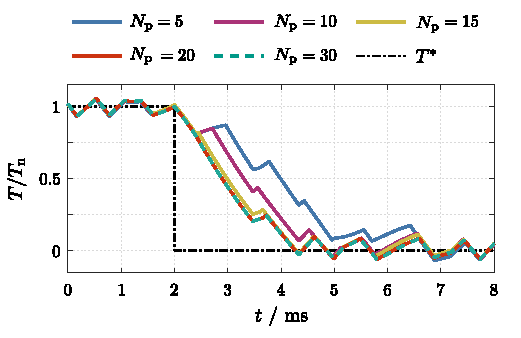
\includegraphics[width=0.65\textwidth]{fig/lec05/MPC_prediction_length_impact_transient.pdf}
        \caption{Transient torque response of a IM drive controlled by FCS-MPC for different prediction horizons $N_\mathrm{p}$ (modified from source: \href{https://ieeexplore.ieee.org/document/9830061}{0.1109/TPEL.2022.3190713}, \href{https://creativecommons.org/licenses/by/4.0/deed.en}{CC BY 4.0}).}
        \label{fig:mpc_horizon_transient}
    \end{figure}
\end{frame}

%%%%%%%%%%%%%%%%%%%%%%%%%%%%%%%%%%%%%%%%%%%%%%%%%%%%%%%%%%%%%
%% Impact of the prediction horizon on performance (cont.) %%
%%%%%%%%%%%%%%%%%%%%%%%%%%%%%%%%%%%%%%%%%%%%%%%%%%%%%%%%%%%%%
\begin{frame}[c]
    \frametitle{Impact of the prediction horizon on performance (cont.)}
    \centering
    \begin{figure}
        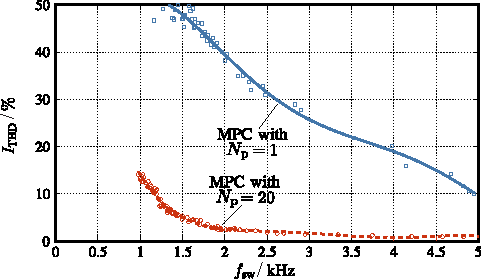
\includegraphics[width=0.65\textwidth]{fig/lec05/MPC_prediction_length_impact_steady_state.pdf}
        \caption{Trade-off curves for different prediction steps $N_\mathrm{p}$ between stator current THD and switching frequency for FCS-MPC addressing an IM drive with LC filter between inverter and motor (modified from source: \href{https://ieeexplore.ieee.org/abstract/document/9180048}{10.1109/OJIA.2020.3020184}, \href{https://creativecommons.org/licenses/by/4.0/deed.en}{CC BY 4.0}).}
        \label{fig:mpc_horizon_steady_state}
    \end{figure}
\end{frame}


%%%%%%%%%%%%%%%%%%%%%%%%%%%%%%%%%%%%%%%%%%%%%%%%%%%%%%%%%%%%%%%%%%
\subsection{Reinforcement learning (RL)}
%%%%%%%%%%%%%%%%%%%%%%%%%%%%%%%%%%%%%%%%%%%%%%%%%%%%%%%%%%%%%%%%%%


%%%%%%%%%%%%%%%%%%%%%%%%%%%%%%%%%%%%%%%%%%%%%%%%%%%%%%%%%%%%%
%% The basic reinforcement learning structure %%
%%%%%%%%%%%%%%%%%%%%%%%%%%%%%%%%%%%%%%%%%%%%%%%%%%%%%%%%%%%%%
\frame{\frametitle{The basic reinforcement learning structure}
    \begin{columns}[t,onlytextwidth]
        \begin{column}{0.6\textwidth}
            \begin{minipage}[c]{\linewidth}
                \begin{figure}
                    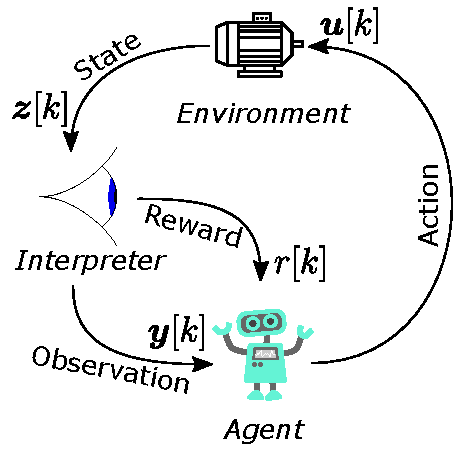
\includegraphics[height=0.6\textheight]{fig/lec05/RL_Wiki.pdf}
                    \caption{The basic RL operation principle\\(derivative of \href{https://commons.wikimedia.org/wiki/File:Reinforcement_learning_diagram.svg}{www.wikipedia.org}, \href{https://creativecommons.org/publicdomain/zero/1.0/deed.en}{CC0 1.0})}
                    \label{fig:RL_Wiki}
                \end{figure}
            \end{minipage}
        \end{column}
        \hfill
        \begin{column}{0.38\textwidth}
            \begin{minipage}[c]{\linewidth}
                \vspace{0.3cm}\pause
                Key characteristics:
                \begin{itemize}
                    \item No supervisor
                    \item Data-driven\pause
                    \item Sequential data stream (not i.i.d. data)
                    \item Agent actions affect subsequent data (sequential decision making)
                \end{itemize}
            \end{minipage}
        \end{column}
    \end{columns}
}

%%%%%%%%%%%%%%%%%%%%%%%%%%%%%%%%%%%%%%%%%%%%%%%%%%%%%%%%%%%%%
%% Reinforcement learning starts from a Markov decision process
%%%%%%%%%%%%%%%%%%%%%%%%%%%%%%%%%%%%%%%%%%%%%%%%%%%%%%%%%%%%%
\begin{frame}
    \frametitle{Reinforcement learning starts from a Markov decision process}
    A sampled control problem can be represented by the \hl{Markov decision process} (MDP)
    \begin{equation}
        \mathcal{M}=(\mathcal{Z},\mathcal{U},p,r_{\mathrm{RL}},\gamma),
        \qquad \gamma\in[0,1),
    \end{equation}
    with (augmented) \hl{MDP state} $\bm{z}[k]\in\mathcal{Z}$ and control action $\bm{u}[k]\in\mathcal{U}$ based on the \hl{policy} $\pi_{\bm{\theta}}$ with parameters $\bm{\theta}$:
    \begin{equation}
        \bm{z}[k+1]\sim p\bigl(\cdot\mid\bm{z}[k],\bm{u}[k]\bigr),
        \qquad
        \bm{u}[k]\sim\pi_{\bm{\theta}}\bigl(\cdot\mid\bm{z}[k]\bigr).
    \end{equation}
    The \hl{discount factor} $\gamma$ weights future rewards: small $\gamma$ emphasizes immediate behavior, while $\gamma\rightarrow 1$ emphasizes long-term consequences.
    For a drive-control tracking task, $\bm{z}[k]$ should include all variables such that the entire information decribing closed-loop behavior is captured, e.g.,
    \begin{equation}
        \bm{z}[k]
        =\begin{bmatrix}
            \bm{x}[k]\T & \bm{r}[k]\T & \bm{u}[k-1]\T
        \end{bmatrix}\T.
    \end{equation}
    Here, $\bm{r}[k]$ remains the control \hl{reference}.
\end{frame}

%%%%%%%%%%%%%%%%%%%%%%%%%%%%%%%%%%%%%%%%%%%%%%%%%%%%%%%%%%%%%
%% Reward function versus stage cost
%%%%%%%%%%%%%%%%%%%%%%%%%%%%%%%%%%%%%%%%%%%%%%%%%%%%%%%%%%%%%
\begin{frame}
    \frametitle{Reward function versus stage cost}
    In RL, the environment returns a scalar \hl{reward} realization
    \begin{equation}
        r_{\mathrm{RL}}[k+1]
        =r_{\mathrm{RL}}\bigl(\bm{z}[k],\bm{u}[k],\bm{z}[k+1]\bigr).
    \end{equation}
    The control agent maximizes accumulated future rewards. For a classical control objective with stage cost $\ell$, a natural choice is
    \begin{equation}
        \boxed{
            r_{\mathrm{RL}}[k+1]
            =-\ell\bigl(\bm{x}[k],\bm{u}[k],\bm{r}[k]\bigr)-p_{\mathrm{c}}[k],}
    \end{equation}
    where $p_{\mathrm{c}}[k]\geq 0$ collects optional \hl{penalties} for constraint violations, e.g., overcurrent or inadmissible voltage usage.
    \begin{block}{Interpretation}
        \begin{equation*}
            \text{small stage cost }\ell \quad\Longleftrightarrow\quad \text{large reward }r_{\mathrm{RL}}.
        \end{equation*}
        If $r_{\mathrm{RL}}=-\ell$ and $p_{\mathrm{c}}=0$, maximizing expected discounted return is equivalent to minimizing the corresponding discounted cost.
    \end{block}
\end{frame}



%%%%%%%%%%%%%%%%%%%%%%%%%%%%%%%%%%%%%%%%%%%%%%%%%%%%%%%%%%%%%
%% Return and action-value function
%%%%%%%%%%%%%%%%%%%%%%%%%%%%%%%%%%%%%%%%%%%%%%%%%%%%%%%%%%%%%
\begin{frame}
    \frametitle{Return and action-value function}
    The \hl{return} from time step $k$ is
    \begin{equation}
        G[k]=\sum_{j=0}^{\infty}\gamma^j r_{\mathrm{RL}}[k+j+1].
    \end{equation}
    For a policy $\pi$, the \hl{value} and \hl{action-value} functions are
    \begin{align}
        v_{\pi}(\bm{z})
         & =\mathbb{E}_{\pi}\bigl[G[k]\mid\bm{z}[k]=\bm{z}\bigr],                  \\
        q_{\pi}(\bm{z},\bm{u})
         & =\mathbb{E}_{\pi}\bigl[G[k]\mid\bm{z}[k]=\bm{z},\bm{u}[k]=\bm{u}\bigr].
    \end{align}
    Hence,
    \begin{equation}
        v_{\pi}(\bm{z})
        =\mathbb{E}_{\bm{u}\sim\pi(\cdot|\bm{z})}
        \left[q_{\pi}(\bm{z},\bm{u})\right].
    \end{equation}
    The \hl{optimal (greedy) policy} is obtained from
    \begin{equation}
        \boxed{\pi^{*}(\bm{z})\in
            \argmax_{\bm{u}\in\mathcal{U}(\bm{z})}
            q^{*}(\bm{z},\bm{u}).}
    \end{equation}
    Thus, $q^{*}$ evaluates each state-action pair by its expected future reward.
\end{frame}

%%%%%%%%%%%%%%%%%%%%%%%%%%%%%%%%%%%%%%%%%%%%%%%%%%%%%%%%%%%%%
%% Bellman optimality and temporal-difference learning
%%%%%%%%%%%%%%%%%%%%%%%%%%%%%%%%%%%%%%%%%%%%%%%%%%%%%%%%%%%%%
\begin{frame}
    \frametitle{Bellman optimality and temporal-difference learning}
    The optimal action-value function satisfies the (recursive) \hl{Bellman optimality equation}
    \begin{equation}
        \boxed{
            q^{*}(\bm{z},\bm{u})
            =\mathbb{E}\left[
                r_{\mathrm{RL}}[k+1]
                +\gamma\max_{\bm{u}'\in\mathcal{U}(\bm{z}')}
                q^{*}(\bm{z}',\bm{u}')
                \right].}
    \end{equation}
    Here, $(\bm{z}',\bm{u}')$ are the next state and action (at time $k+1$), respectively. For a \hl{parameterized approximation} $q_{\bm{w}}\approx q^{*}$, the temporal-difference target is
    \begin{equation}
        y=r_{\mathrm{RL}}[k+1]
        +\gamma\max_{\bm{u}'}
        q_{\bar{\bm{w}}}(\bm{z}',\bm{u}'),
    \end{equation}
    and the critic loss is
    \begin{equation}
        \mathcal{L}_{q}(\bm{w})
        =\mathbb{E}_{(\bm{z},\bm{u},r_{\mathrm{RL}},\bm{z}')\sim\mathcal{D}}
        \left[\left(q_{\bm{w}}(\bm{z},\bm{u})-y\right)^2\right].
    \end{equation}
    Here, $\mathcal{D}$ is a \hl{replay (data) buffer} and $q_{\bar{\bm{w}}}$ is a slowly updated \hl{target network}. Hence, the loss is the mean-squared error of the estimator's output plugged into the Bellman optimality equation.
\end{frame}

%%%%%%%%%%%%%%%%%%%%%%%%%%%%%%%%%%%%%%%%%%%%%%%%%%%%%%%%%%%%%
%% Deep Q-network for finite-control-set drive control
%%%%%%%%%%%%%%%%%%%%%%%%%%%%%%%%%%%%%%%%%%%%%%%%%%%%%%%%%%%%%
\begin{frame}
    \frametitle{Deep Q-network for finite-control-set drive control}
    For a two-level inverter, the finite RL control action is the switching state
    \begin{equation}
        \bm{u}[k]=\bm{s}[k]\in\mathbb{S}
        =\{\bm{s}_0,\ldots,\bm{s}_7\}.
    \end{equation}
    A \hl{deep Q-network} (DQN) maps the MDP state to one return estimate per switching action:
    \begin{equation}
        q_{\bm{w}}(\bm{z},\cdot)
        =\begin{bmatrix}
            q_{\bm{w}}(\bm{z},\bm{s}_0) & \cdots & q_{\bm{w}}(\bm{z},\bm{s}_7)
        \end{bmatrix}\T.
    \end{equation}\vspace{-0.3cm}
    \begin{columns}[c]
        \begin{column}{0.55\textwidth}
            \onslide<4->{
                    \begin{block}{FCS-RL solution}
                        Once an accurate estimate $q_{\bm{w}}$ is found, the optimal action / policy is easily determined and the task is solved: just compare the finite $n_{\mathrm{s}}$ outputs of the estimator and select the best one:
                        \begin{equation}
                            \bm{s}^{*}[k]
                            \in\argmax_{\bm{s}_i\in\mathbb{S}}
                            q_{\bm{w}}^{*}\bigl(\bm{z}[k],\bm{s}_i\bigr).
                        \end{equation}
                    \end{block}}
        \end{column}
        \begin{column}[c]{0.45\textwidth}
            \centering
            \onslide<2->{
                    \begin{tikzpicture}[
                            process/.style={rectangle, rounded corners, minimum width=1.6cm, minimum height=1.5cm, text centered, draw=black, fill=gray!40, font=\footnotesize, align = center},
                        ]
                        \node[process] (ann) {Estimator\\[1em]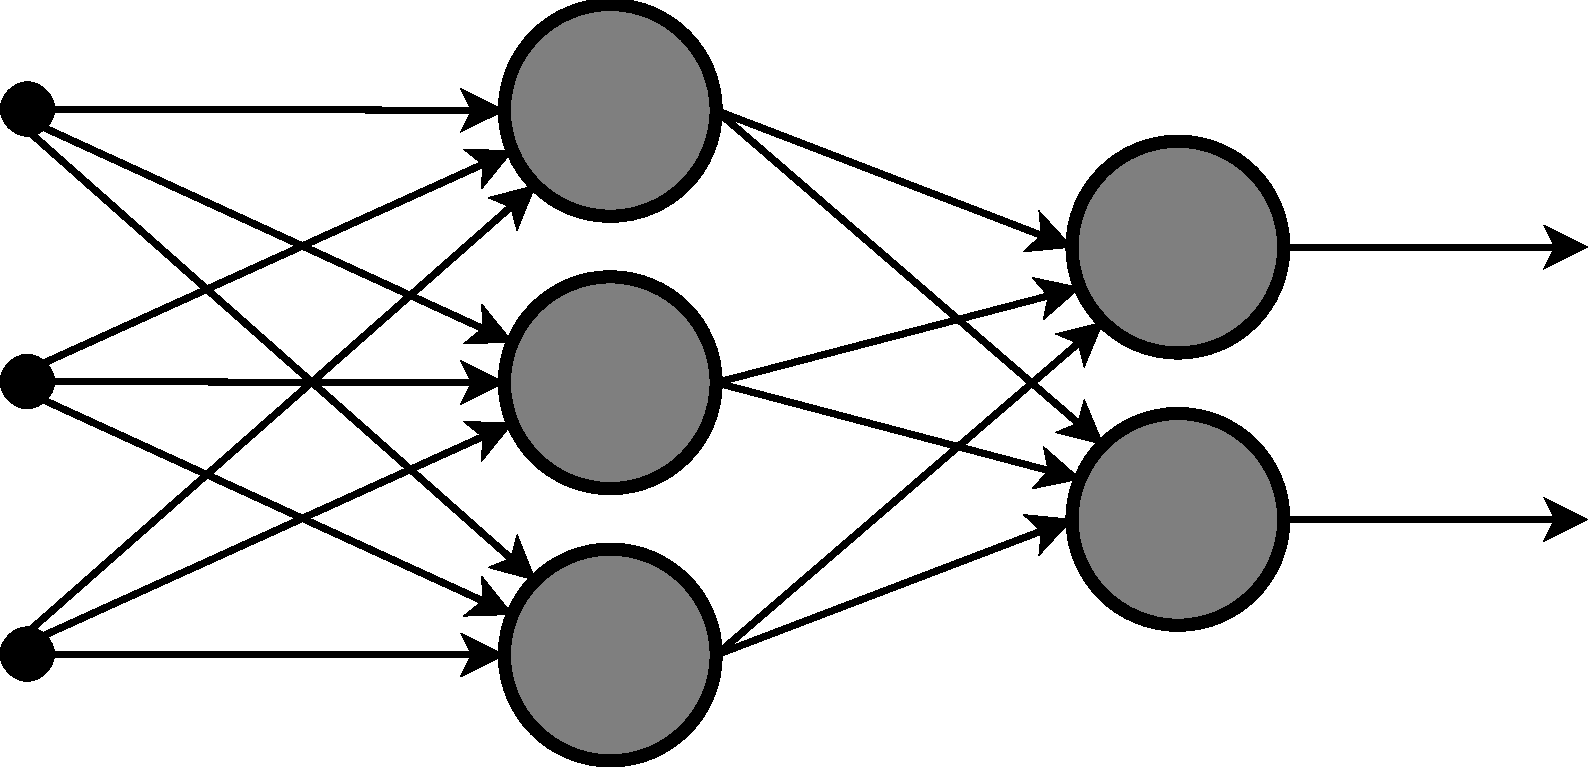
\includegraphics[width=1.25cm]{fig/lec05/ANN_symbol.pdf}};
                        \draw[<-] (ann.west) -- ++(-1,0) node[midway, above]{$\bm{z}[k]$};
                        \foreach \i in {0.2, 0.4, 0.6, 0.8} {
                                \draw[->] ($(ann.north east)!\i!(ann.south east)$) to ++(1,0);
                            }
                        \node[right] at ($(ann.east) + (1,0)$) {$q_{\bm{w}}(\bm{z}[k], \bm{s}_{i=1,\ldots})$};
                    \end{tikzpicture}}
        \end{column}
    \end{columns}
\end{frame}

%%%%%%%%%%%%%%%%%%%%%%%%%%%%%%%%%%%%%%%%%%%%%%%%%%%%%%%%%%%%%
%% Summary of DQN Working Principle  %%
%%%%%%%%%%%%%%%%%%%%%%%%%%%%%%%%%%%%%%%%%%%%%%%%%%%%%%%%%%%%%
\frame{\frametitle{Summary of DQN working principle }
    \begin{figure}
        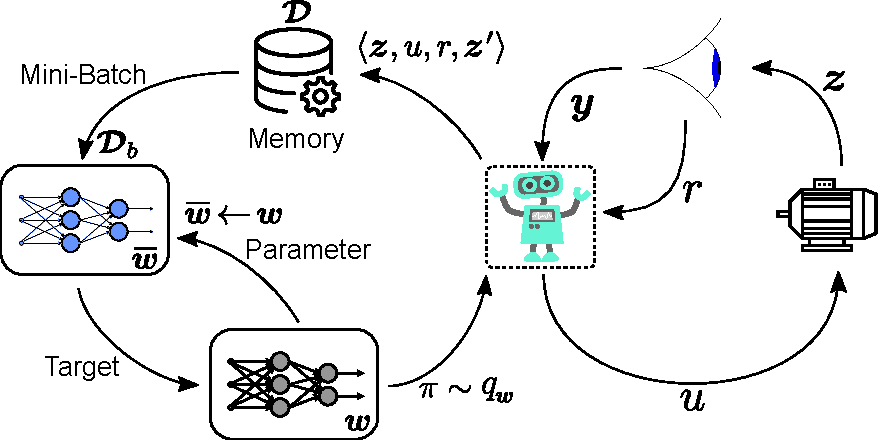
\includegraphics[height=5.5cm]{fig/lec05/DQN.pdf}
        \caption{DQN structure from a bird's-eye perspective (derivative work of \figref{fig:RL_Wiki} and \href{https://commons.wikimedia.org/wiki/File:Multi-Layer_Neural_Network-Vector.svg?uselang=de}{wikipedia.org}, \href{https://creativecommons.org/publicdomain/zero/1.0/deed.en}{CC0 1.0})}
        \label{fig:DQN}
    \end{figure}
}

%%%%%%%%%%%%%%%%%%%%%%%%%%%%%%%%%%%%%%%%%%%%%%%%%%%%%%%%%%%%%
%% DQN training loop and control-specific challenges
%%%%%%%%%%%%%%%%%%%%%%%%%%%%%%%%%%%%%%%%%%%%%%%%%%%%%%%%%%%%%
\begin{frame}
    \frametitle{DQN training loop and control-specific challenges}
    To improve the policy over time the agent needs to apply \hl{exploration} to receive new data deviating from the current greedy policy. A simple $\varepsilon$-greedy exploration strategy is
    \begin{equation*}
        \bm{s}[k]=
        \begin{cases}
            \text{random admissible switching action},                                  & \text{with probability }\varepsilon, \\
            \displaystyle\argmax_{\bm{s}_i\in\mathbb{S}}q_{\bm{w}}(\bm{z}[k],\bm{s}_i), & \text{otherwise}.
        \end{cases}
    \end{equation*}
    Additional thoughts for drive control:
    \begin{itemize}
        \item enforce hard constraints by action masking, safety filters, or constrained training,
        \item include $\bm{s}[k-1]$ in $\bm{z}[k]$ when switching transitions are penalized,
        \item cover relevant operating points to limit extrapolation risk,
        \item note that a learned DQN has no  optimality guarantee (need for empirical validation).
    \end{itemize}
\end{frame}

%%%%%%%%%%%%%%%%%%%%%%%%%%%%%%%%%%%%%%%%%%%%%%%%%%%%%%%%%%%%%
%% Continuous actions motivate actor-critic methods
%%%%%%%%%%%%%%%%%%%%%%%%%%%%%%%%%%%%%%%%%%%%%%%%%%%%%%%%%%%%%
\begin{frame}
    \frametitle{Continuous actions motivate actor-critic methods}
    For CCS control, the RL action is a continuous vector (e.g., stator voltage in dq frame):
    \begin{equation*}
        \bm{u}[k]\in\mathcal{U}_{\mathrm{CCS}}.
    \end{equation*}
    A value-only method would require solving a continuous NLP
    \begin{equation*}
        \bm{u}^{*}(\bm{z})
        \in\argmax_{\bm{u}\in\mathcal{U}_{\mathrm{CCS}}}
        q_{\bm{w}}(\bm{z},\bm{u})
    \end{equation*}
    at every sampling instant. \hl{Actor-critic methods} avoid this inner optimization by learning a \hl{direct / explicit mapping} from state to actions:
    \begin{equation*}
        \underbrace{\bm{u}=\bm{\pi}_{\bm{\theta}}(\bm{z})}_{\text{actor: direct control action}},
        \qquad
        \underbrace{q_{\bm{w}}(\bm{z},\bm{u})}_{\text{critic: evaluates the action}}.
    \end{equation*}
    \begin{center}
        \begin{tikzpicture}[>=Latex,node distance=7mm and 8mm,scale=0.94,transform shape,
                box/.style={draw,rounded corners,minimum height=9mm,minimum width=26mm,align=center,font=\scriptsize}]
            \node[box] (state) {MDP state\\$\bm{z}$};
            \node[box,right=of state] (actor) {actor\\$\bm{\pi}_{\bm{\theta}}$};
            \node[box,right=of actor] (action) {continuous action\\$\bm{u}$};
            \node[box,below=8mm of actor] (critic) {critic\\$q_{\bm{w}}(\bm{z},\bm{u})$};
            \draw[-Latex] (state)--(actor);
            \draw[-Latex] (actor)--(action);
            \draw[-Latex] (state.south) |- (critic.west);
            \draw[-Latex] (action.south) |- (critic.east);
            \draw[-Latex,dashed] (critic.north)--(actor.south);
        \end{tikzpicture}
    \end{center}
\end{frame}


%%%%%%%%%%%%%%%%%%%%%%%%%%%%%%%%%%%%%%%%%%%%%%%%%%%%%%%%%%%%%
%% Deterministic actor-critic learning
%%%%%%%%%%%%%%%%%%%%%%%%%%%%%%%%%%%%%%%%%%%%%%%%%%%%%%%%%%%%%
\begin{frame}
    \frametitle{Deterministic actor-critic learning for continuous actions}
    For a \hl{differentiable deterministic policy} $\bm{\pi}_{\bm{\theta}}(\bm{z})=\bm{\mu}_{\bm{\theta}}(\bm{z})$, define the expected return as evaluation metric:
    \begin{equation*}
        J(\bm{\theta})=\mathbb{E}_{\bm{\mu}_{\bm{\theta}}}\left[G[0]\right]
        \quad\longrightarrow\quad \max_{\bm{\theta}}.
    \end{equation*}
    For a deterministic actor $\bm{u}=\bm{\mu}_{\bm{\theta}}(\bm{z})$, the \hl{critic} is trained from
    \begin{equation*}
        y=r_{\mathrm{RL}}[k+1]
        +\gamma q_{\bar{\bm{w}}}
        \bigl(\bm{z}',\bm{\mu}_{\bar{\bm{\theta}}}(\bm{z}')\bigr),
    \end{equation*}
    with
    \begin{equation*}
        \mathcal{L}_{q}(\bm{w})
        =\mathbb{E}_{\mathcal{D}}
        \left[\left(q_{\bm{w}}(\bm{z},\bm{u})-y\right)^2\right].
    \end{equation*}
    The \hl{deterministic policy gradient} is
    \begin{equation*}
        \boxed{
            \nabla_{\bm{\theta}}J(\bm{\theta})
            \approx
            \mathbb{E}_{\bm{z}\sim\mathcal{D}}
            \left[
                \nabla_{\bm{\theta}}\bm{\mu}_{\bm{\theta}}(\bm{z})
                \,\nabla_{\bm{u}}q_{\bm{w}}(\bm{z},\bm{u})
                \big|_{\bm{u}=\bm{\mu}_{\bm{\theta}}(\bm{z})}
                \right].}
    \end{equation*}
    Voltage constraints can be encoded by projection or a bounded output map, e.g.,
    \begin{equation*}
        \bm{u}
        =\operatorname{proj}_{\mathcal{U}_{\mathrm{CCS}}}
        \bigl(\bm{\mu}_{\bm{\theta}}(\bm{z})\bigr).
    \end{equation*}
\end{frame}

%%%%%%%%%%%%%%%%%%%%%%%%%%%%%%%%%%%%%%%%%%%%%%%%%%%%%%%%%%%%%
%% Summary of DQN Working Principle  (2)%%
%%%%%%%%%%%%%%%%%%%%%%%%%%%%%%%%%%%%%%%%%%%%%%%%%%%%%%%%%%%%%
\frame{\frametitle{Visual summary of DDPG working principle}
    \begin{figure}
        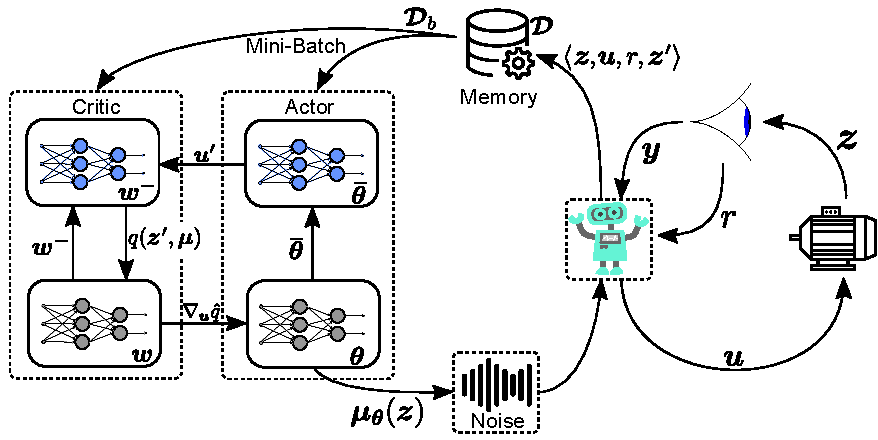
\includegraphics[height=5.75cm]{fig/lec05/DDPG.pdf}
        \caption{DDPG structure from a bird's-eye perspective (derivative work of \figref{fig:RL_Wiki} and \href{https://commons.wikimedia.org/wiki/File:Multi-Layer_Neural_Network-Vector.svg?uselang=de}{wikipedia.org}, \href{https://creativecommons.org/publicdomain/zero/1.0/deed.en}{CC0 1.0})}
        \label{fig:DDPG}
    \end{figure}
}

%%%%%%%%%%%%%%%%%%%%%%%%%%%%%%%%%%%%%%%%%%%%%%%%%%%%%%%%%%%%%
%% Reinforcement learning starts from a Markov decision process0
%%%%%%%%%%%%%%%%%%%%%%%%%%%%%%%%%%%%%%%%%%%%%%%%%%%%%%%%%%%%%
\begin{frame}
    \frametitle{RL methods for finite and continuous control sets (in drive control)}
    \begin{center}
        \begin{tabular}{p{0.25\textwidth}p{0.31\textwidth}p{0.34\textwidth}}
            \toprule
                                   & \textbf{Finite control set}                      & \textbf{Continuous control set}                                \\
            \midrule
            Action                 & $\bm{s}_i\in\mathbb{S}$                          & $\bm{u}_{\mathrm{s},\mathrm{dq}}\in\mathcal{U}_{\mathrm{CCS}}$ \\[1mm]
            Main approximation     & $q^{*}(\bm{z},\bm{s}_i)$                         & actor $\bm{\mu}_{\bm{\theta}}$ and critic $q_{\bm{w}}$         \\[1mm]
            Online operation       & finite $\argmax$ over $q_{\bm{w}}(\bm{z},\cdot)$ & direct actor $\bm{\mu}_{\bm{\theta}}$ evaluation               \\[1mm]
            Representative methods & DQN, Rainbow                                     & DDPG, TD3, SAC, PPO                                            \\
            \bottomrule
        \end{tabular}
    \end{center}

    \begin{block}{Further study}
        A complete open course with slides, videos, tutorial templates, and solutions is available at
        \begin{center}
            \href{https://github.com/IAS-Uni-Siegen/RL_course}
            {\textbf{github.com/IAS-Uni-Siegen/RL\_course}}
        \end{center}
        Topics include MDPs, temporal-difference learning, value-based control, policy gradients, and actor-critic methods.
    \end{block}
\end{frame}

%%%%%%%%%%%%%%%%%%%%%%%%%%%%%%%%%%%%%%%%%%%%%%%%%%%%%%%%%%%%%%%%%%
\subsection{Differentiable predictive control (DPC)}
%%%%%%%%%%%%%%%%%%%%%%%%%%%%%%%%%%%%%%%%%%%%%%%%%%%%%%%%%%%%%%%%%%


%%%%%%%%%%%%%%%%%%%%%%%%%%%%%%%%%%%%%%%%%%%%%%%%%%%%%%%%%%%%%
%% Comparison of approximation methods%%
%%%%%%%%%%%%%%%%%%%%%%%%%%%%%%%%%%%%%%%%%%%%%%%%%%%%%%%%%%%%%
\begin{frame}
    \frametitle{Comparison of approximation methods}
    \begin{center}
        \begin{tabular}{P{0.15\textwidth}P{0.2\textwidth}P{0.55\textwidth}}
            \toprule
            \textbf{Method} & \textbf{Online operation}           & \textbf{Main approximation}                           \\
            \midrule
            MPC             & solve \eqref{eq:mpc_ocp}            & infinite horizon $\rightarrow$ finite horizon         \\
            RL              & evaluate $\bm{\pi}_{\bm{\theta}^*}$ & Bellman solution $\rightarrow$ learned value / policy \\
            DPC             & evaluate $\bm{\pi}_{\bm{\theta}^*}$ & closed-loop rollouts $\rightarrow$ trained feedback   \\
            \bottomrule
        \end{tabular}
    \end{center}
    \begin{varblock}{A few final remarks}
        The above summaries are intended to provide a high-level overview of the main ideas -- important aspects, like recursive feasibility and safety guarantees, are not covered. Further important but uncovered aspects are the training and deployment strategies (offline vs. online, simulation vs. real-world, etc.) and the choice of the function approximator (e.g., neural network architecture). If handled carefully, all three methods can be used to achieve high-performance drive control close to the physical limits of the system.
    \end{varblock}
\end{frame}


